\chapter{Desenvolvimento}
Neste capítulo serão abordados diversos aspectos do desenvolvimento do sistema, desde a configuração do ambiente de desenvolvimento até o fluxo de trabalho utilizado durante o processo de criação da aplicação. Serão apresentados os desafios encontrados durante o desenvolvimento, bem como as soluções adotadas para superá-los, além de uma visão geral sobre as funcionalidades do sistema e as tecnologias utilizadas para sua criação.

\section{Especificação de requisitos}\label{sec:especificacao_de_requisitos}
% Descrever os requisitos funcionais e não funcionais da aplicação móvel, incluindo as funcionalidades que ela deve ter e as plataformas em que deve ser executada.
O pontapé inicial do projeto foi uma reunião entre as partes envolvidas, cliente (docentes de Agronomia da \ac{ufape}), \ac{po} (Proprietário do produto, em tradução livre) e desenvolvedores, a fim de levantar os requisitos funcionais do \ac{mvp}. Nesta reunião foram explanados os pontos onde o \ac{app} auxiliaria no gerenciamento de experimentos e no processo dos cálculos enzimáticos, foram discutidas regras de negócios e requisitos necessários, identidade visual, além do início de um protótipo de baixa fidelidade para conduzir o \textit{brainstorming} a respeito de como os requisitos se transformariam em funcionalidades, e claro, as tecnologias utilizadas em todo o ciclo de desenvolvimento.

O projeto surge com necessidade de um \ac{app} para celulares, facilitando a mobilidade dos usuários nos locais de coletas de dados para os experimentos, dessa forma, tudo foi pensado voltado ao desenvolvimento deste aplicativo móvel.

\subsection{Requisitos funcionais}\label{ssec:requisitos_funcionais}
A partir disso, os requisitos funcionais do sistema foram definidos e especificados de acordo com a \tabref{table:requisitos_funcionais}, abaixo.

\begin{table}[H]
\centering
\resizebox{\textwidth}{!}{%
\begin{tabular}{|l|l|}
\hline
\textbf{Código} & \textbf{Descrição} \\ \hline
RF01   & O usuário deve ser capaz de se cadastrar no sistema \\ \hline
RF02   & O usuário deve ser capaz de realizar \textit{login} no sistema \\ \hline
RF03   & O usuário deve ser capaz de recuperar sua senha no sistema \\ \hline
RF04   & O usuário deve ser capaz de criar um tratamento \\ \hline
RF05   & O usuário deve ser capaz de deletar um tratamento \\ \hline
RF06   & \vtop{\hbox{\strut O usuário deve ser capaz de visualizar todos os tratamentos disponíveis}\hbox{\strut no sistema para seus experimentos}} \\ \hline
RF07   & O usuário administrador deve ser capaz de criar uma nova enzima \\ \hline
RF08   & O usuário administrador deve ser capaz de deletar uma enzima \\ \hline
RF09   & \vtop{\hbox{\strut O usuário deve ser capaz de visualizar todas as enzimas disponíveis}\hbox{\strut no sistema para seus experimentos}} \\ \hline
RF10   & O usuário deve ser capaz de criar um novo experimento \\ \hline
RF11   & O usuário deve ser capaz de deletar um experimento \\ \hline
RF12   & O usuário deve ser capaz de visualizar seus experimentos cadastrados \\ \hline
RF13   & \vtop{\hbox{\strut O usuário deve ser capaz de utilizar filtros de busca}\hbox{\strut para visualizar seus experimentos cadastrados}} \\ \hline
RF14   & O usuário deve ser capaz de visualizar detalhes dos seus experimentos cadastrados \\ \hline
RF15   & \vtop{\hbox{\strut O usuário deve ser capaz de inserir dados para o cálculo enzimático}\hbox{\strut no seu experimento}} \\ \hline
RF16   & \vtop{\hbox{\strut O usuário deve ser capaz de visualizar resultados discrepantes do cálculo}\hbox{\strut enzimático antes de salvar no seu experimento}}  \\ \hline
RF17   & \vtop{\hbox{\strut O usuário deve ser capaz de editar o resultado do cálculo enzimático}\hbox{\strut antes de salvar no seu experimento}} \\ \hline
RF18   & \vtop{\hbox{\strut O usuário deve ser capaz de salvar o resultado do cálculo enzimático}\hbox{\strut no seu experimento}} \\ \hline
RF19   & \vtop{\hbox{\strut O usuário deve ser capaz de visualizar os resultados e o progresso}\hbox{\strut do seu experimento}} \\ \hline
RF20   & O usuário deve ser capaz de exportar os resultados do seu experimento  \\ \hline

\end{tabular}%
}
\caption{Descrição dos requisitos funcionais do sistema}
\label{table:requisitos_funcionais}
\end{table}

Segundo \cite{pressman2016engenharia}, os requisitos funcionais, que descrevem as funções e serviços que o software deve oferecer, descrevem como o software deve funcionar, quais entradas devem ser processadas e quais saídas devem ser geradas em resposta a essas entradas. Neste sentido, os requisitos funcionais descritos na \tabref{table:requisitos_funcionais} têm o objetivo de especificar as funcionalidades que o sistema proposto deve oferecer.

\subsection{Casos de uso}\label{ssec:casos_de_uso}

Os Casos de Uso (\textit{Use Cases}) são uma técnica de modelagem de requisitos de software que descrevem as interações entre o usuário e o sistema. Eles ajudam a identificar as funcionalidades e serviços que o software deve oferecer, além de fornecer um meio de comunicação claro entre as equipes de desenvolvimento e os \textit{stakeholders}. A partir disto, foi elaborado um conjunto de casos de uso do sistema, demonstrado na \tabref{table:casos_de_uso}, com o objetivo de centrar os requisitos funcionais descritos na \tabref{table:requisitos_funcionais} e relacionar os mesmos com os tipos de usuários do sistema.

\begin{table}[H]
\centering
\resizebox{\textwidth}{!}{%
\begin{tabular}{|l|l|l|l|}
\hline
\textbf{Código} & \textbf{Descrição} & \textbf{Tipo de usuário} & \textbf{\vtop{\hbox{\strut Requisitos funcionais}\hbox{\strut contemplados}}}\\ \hline
UC01 & Fazer cadastro no sistema & \vtop{\hbox{\strut Usuário comum,}\hbox{\strut Administrador}} & RF01 \\ \hline
UC02 & Fazer \textit{login} no sistema & \vtop{\hbox{\strut Usuário comum,}\hbox{\strut Administrador}} & RF02 \\ \hline
UC03 & Recuperar senha no sistema & \vtop{\hbox{\strut Usuário comum,}\hbox{\strut Administrador}} & RF03 \\ \hline
UC04 & Criar, deletar, visualizar e usar tratamentos & \vtop{\hbox{\strut Usuário comum,}\hbox{\strut Administrador}} & RF04, RF05 e RF06 \\ \hline
UC05 & Criar e deletar enzimas & Administrador & RF07 e RF08 \\ \hline
UC06 & Visualizar e usar enzimas & \vtop{\hbox{\strut Usuário comum,}\hbox{\strut Administrador}} & RF09 \\ \hline
UC07 & Criar, deletar, filtrar e visualizar experimentos & \vtop{\hbox{\strut Usuário comum,}\hbox{\strut Administrador}} &  RF10, RF11, RF12 e RF13 \\ \hline
UC08 & Visualizar detalhes do experimento & \vtop{\hbox{\strut Usuário comum,}\hbox{\strut Administrador}} & RF14 \\ \hline
UC09 & \vtop{\hbox{\strut Inserir dados, editar e salvar o}\hbox{\strut cálculo enzimático no experimento}} & \vtop{\hbox{\strut Usuário comum,}\hbox{\strut Administrador}} & RF15, RF16, RF17 e RF18 \\ \hline
UC10 & Visualizar resultados do experimento & \vtop{\hbox{\strut Usuário comum,}\hbox{\strut Administrador}} & RF19 \\ \hline
UC11 & Compartilhar resultados do experimento & \vtop{\hbox{\strut Usuário comum,}\hbox{\strut Administrador}} & RF20 \\ \hline

\end{tabular}
}
\caption{Casos de Uso do sistema}
\label{table:casos_de_uso}
\end{table}

Uma reprodução visual dos Casos de Uso apontados na \tabref{table:casos_de_uso} e as suas interações com os usuários foi elaborada, na \figref{fig:use-cases-enzitech}. Este diagrama utiliza \ac{uml} — em português: Linguagem de Modelagem Unificada — uma linguagem para visualização, especificação, construção e documentação de artefatos de um software em desenvolvimento, desta forma o Diagrama de \textit{Use Cases} \footnote{Diagrama de \textit{Use Cases}: \url{http://www.dsc.ufcg.edu.br/~jacques/cursos/map/html/uml/diagramas/usecases/usecases.htm}} utilizado abaixo tem o objetivo de auxiliar a comunicação entre os analistas e o cliente, descrevendo um cenário que mostra as funcionalidades do sistema do ponto de vista do usuário. O cliente deve ver neste diagrama as principais funcionalidades de seu sistema.

\begin{figure}[H]
\centering
  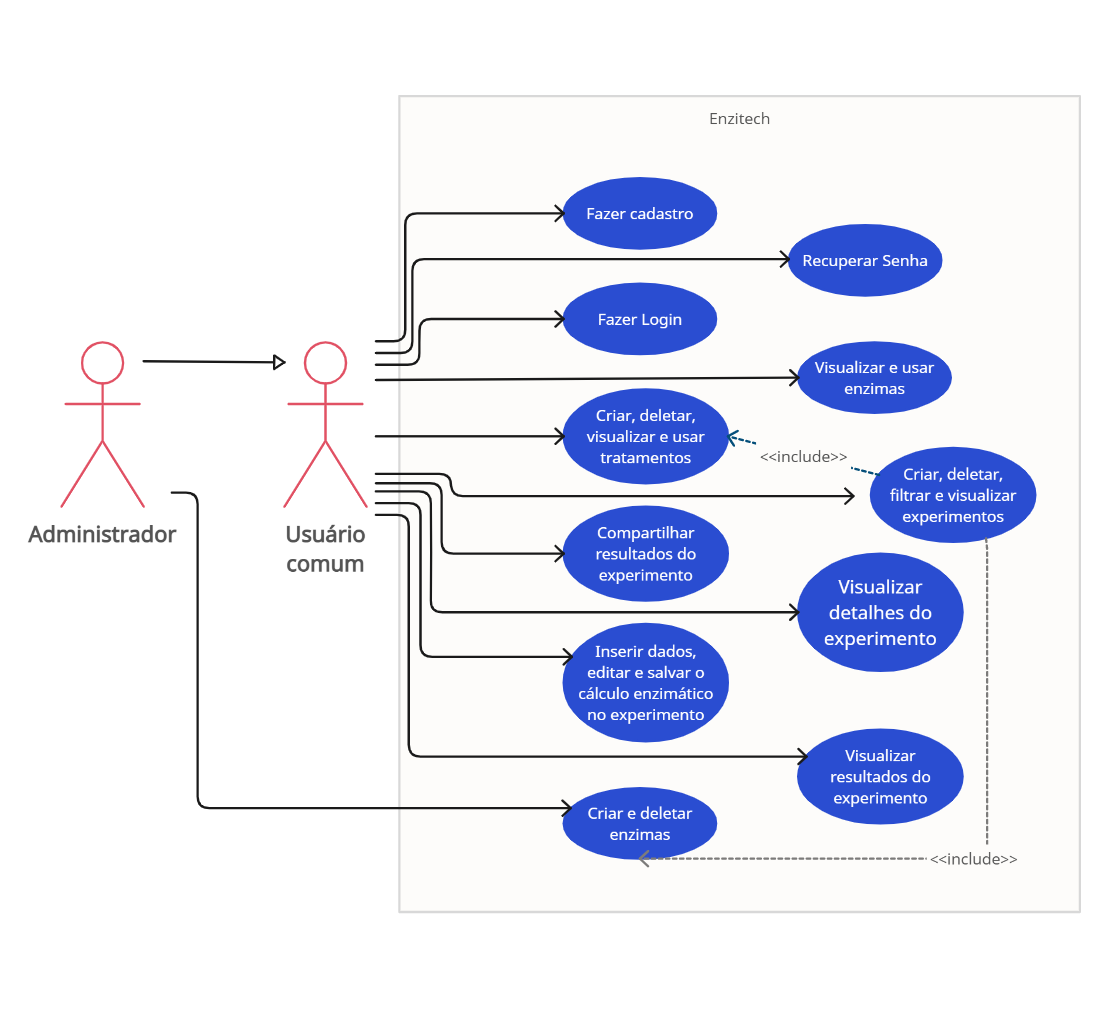
\includegraphics[width=\columnwidth]{images/use-cases-enzitech.png}
  \caption{Diagrama de Casos de Uso do sistema.}
  % \acsfont{Fonte: Autoria própria}
  \label{fig:use-cases-enzitech}
\end{figure}

Graças ao diagrama acima, é possível notar, de forma simples, que um usuário administrador possui um privilégio em comparação ao usuário comum: a criação e exclusão das enzimas, este Caso de Uso que ficou restrito à administração do sistema por ser compartilhada entre todos os usuários do Enzitech, podendo causar perdas de dados se sua alteração for realizada por um usuário comum, portando, surgiu a necessidade de diferenciar ambos os tipos de usuários no sistema e realizar estas validações para a disponibilização dessa \textit{feature}. 

\section{Protótipo}
\cite{warfel2009prototyping} destaca que os protótipos de baixa fidelidade são rápidos e baratos de criar, permitindo que os \textit{designers} testem e refinem rapidamente ideias iniciais. Já os protótipos de alta fidelidade, embora mais caros e demorados, podem ajudar a obter \textit{feedback} mais preciso e detalhado sobre o \textit{design} e a usabilidade do software.

Dentre as diversas reuniões do projeto, houve a discussão das funcionalidades para gerar um protótipo de baixa fidelidade, para possíveis refinamentos, antes da elaboração de um protótipo de alta fidelidade, que demanda mais tempo e esforço. Junto desse protótipo, foi idealizado a identidade visual e o nome oficial para o projeto, que passou a se chamar "Enzitech".

\begin{figure}[H]
\centering
  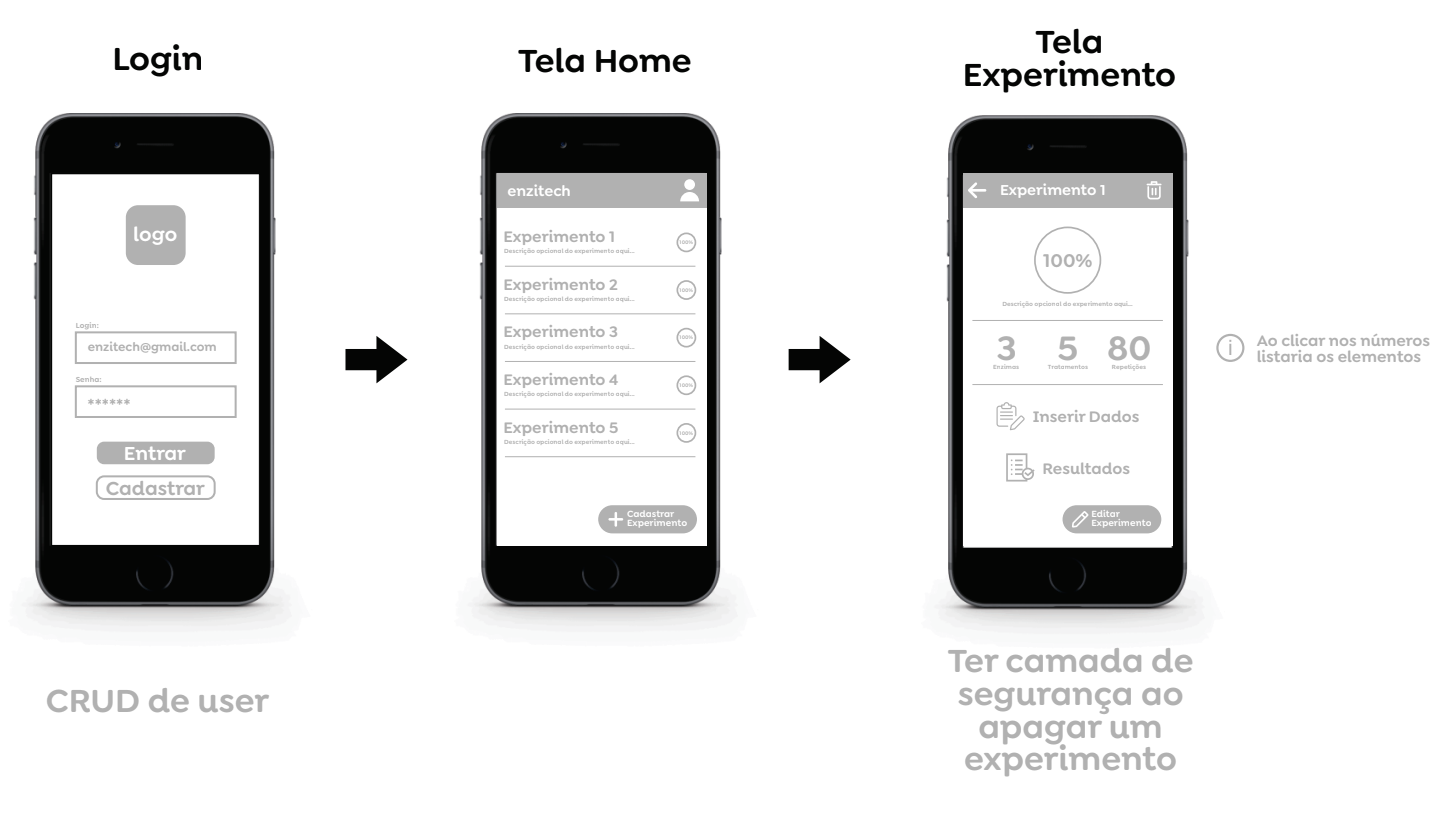
\includegraphics[width=\columnwidth]{images/prototipo_baixa.png}
  \caption{Protótipo final de baixa fidelidade.}
  % \acsfont{Fonte: Autoria própria}
  \label{fig:prototipo_baixa}
\end{figure}

Como é possível ver na \figref{fig:prototipo_baixa}, o protótipo de baixa fidelidade trás o desenho das principais funcionalidades do sistema, além de dar uma ideia do layout final da aplicação.

\begin{figure}[H]
\centering
  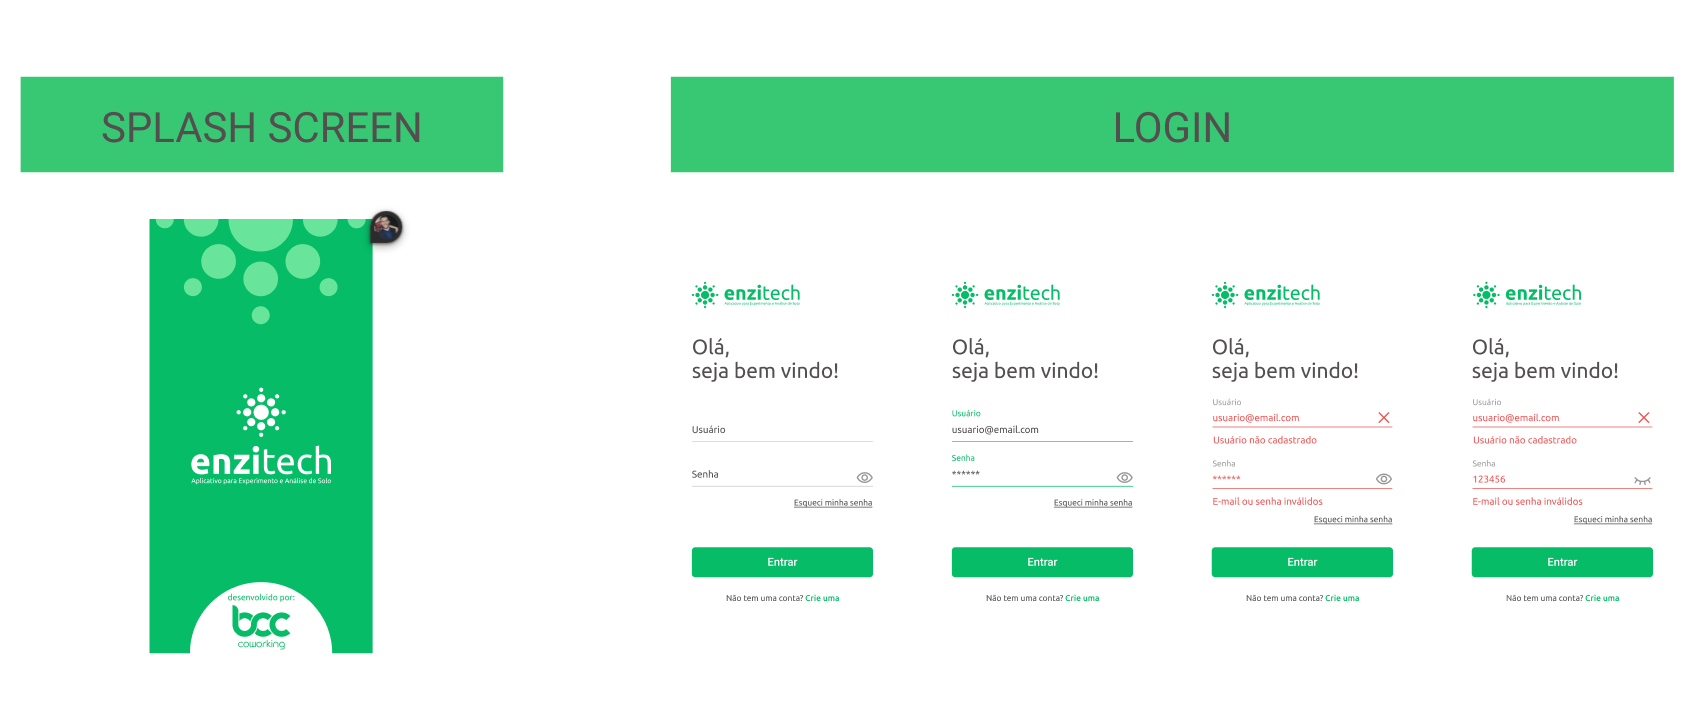
\includegraphics[width=\columnwidth]{images/exemplo_prototipo_alta.png}
  \caption{Parte do protótipo final de alta fidelidade.}
  % \acsfont{Fonte: Autoria própria}
  \label{fig:exemplo_prototipo_alta}
\end{figure}

Já nas \figref{fig:exemplo_prototipo_alta} e \figref{fig:prototipo_alta}, é possível verificar mais a fundo todo o \textit{design-system} aplicado, averiguar comportamentos das telas, fluxo de navegação, entre outras vantagens, trazendo uma versão muito mais refinada da aplicação, auxiliando o desenvolvimento e facilitando a visão do sistema para o cliente, onde antes era definido somente por Casos de Uso.

\begin{figure}[H]
\centering
  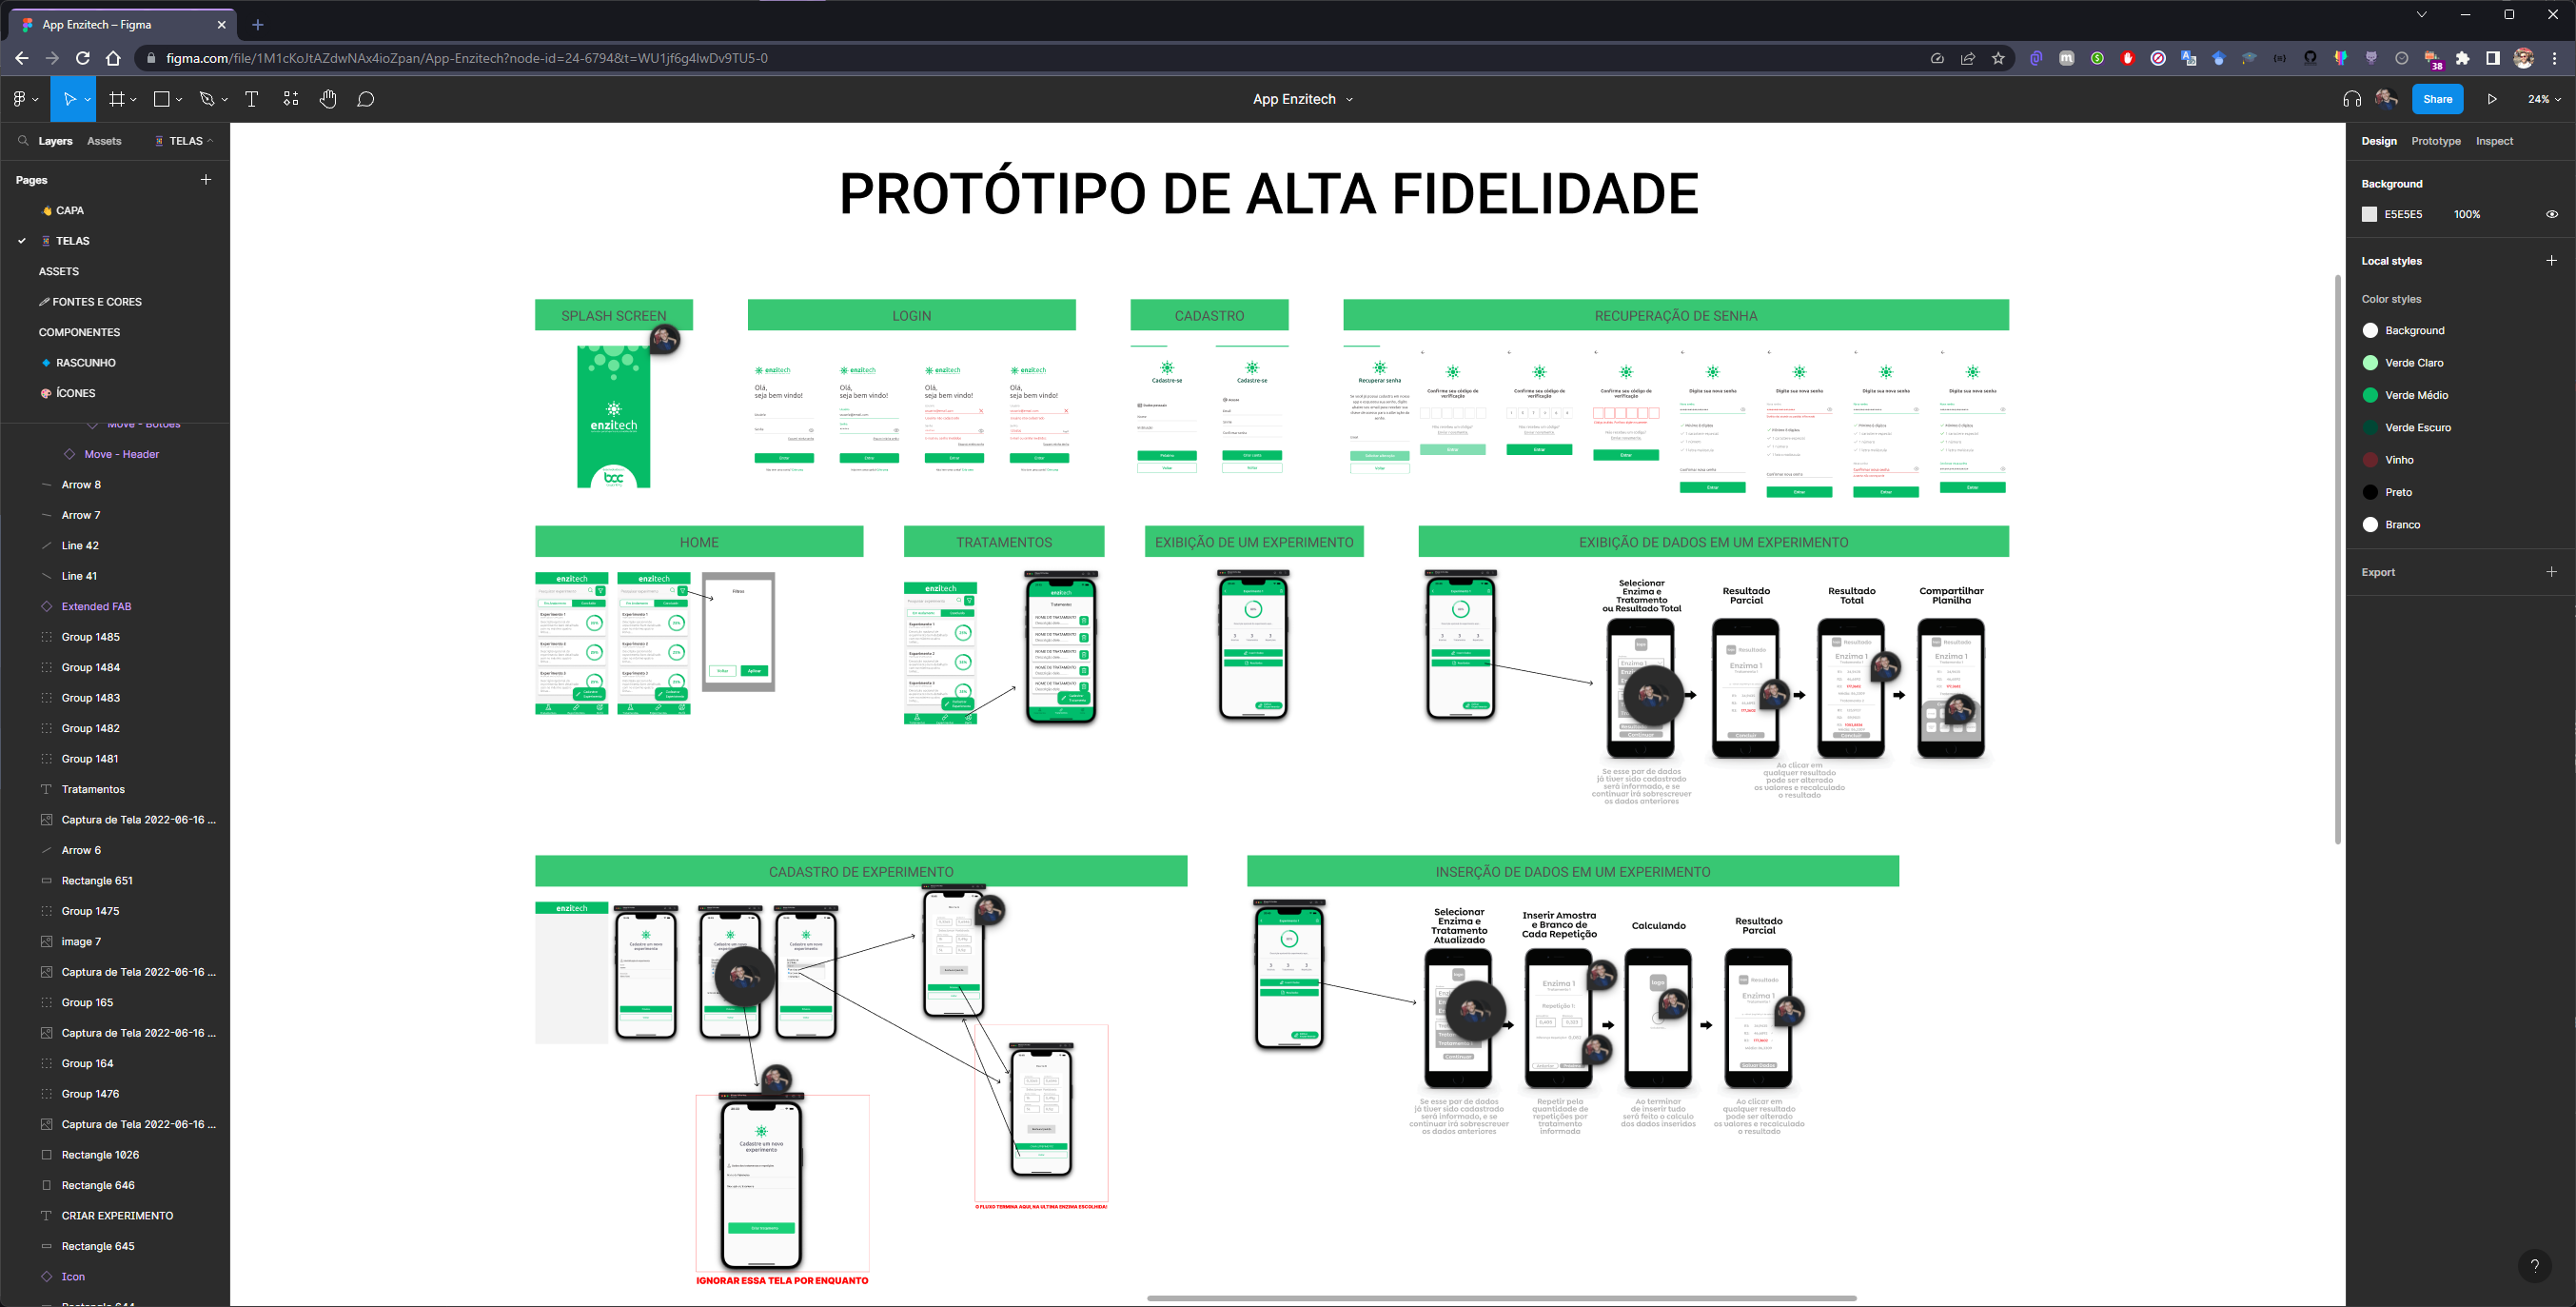
\includegraphics[width=\columnwidth]{images/prototipo_alta.png}
  \caption{Visão geral do protótipo final de alta fidelidade.}
  % \acsfont{Fonte: Autoria própria}
  \label{fig:prototipo_alta}
\end{figure}


\section{Detalhes técnicos do aplicativo}\label{sec:detalhes_tec}
Nesta seção, serão apresentados aspectos como tecnologias utilizadas, os passos necessários para a configuração do ambiente de desenvolvimento, a instalação do Flutter, ferramentas e bibliotecas utilizadas, integrações, gerenciamento de dependências, modelos de dados e o fluxo de trabalho.

\subsection{Instalação do Flutter}\label{ssec:instalacao_flutter}
% Instalação do Flutter e configuração do ambiente de desenvolvimento: Aqui, é importante descrever os passos necessários para instalar o Flutter e configurar o ambiente de desenvolvimento, incluindo a instalação do Android Studio, do emulador Android e da SDK do Android.
Antes de tudo, é necessário elucidar os requisitos para montar um ambiente de desenvolvimento voltado à criação de \acp{app} em Flutter, este \ac{sdk} está disponível nos principais \acp{so} de \acp{pc}, ChromeOS, macOS, Linux e Windows, sendo este último o escolhido como ambiente para o desenvolvimento desta aplicação, o qual será explicado o processo de instalação aqui.

De acordo com o site oficial\footnote{\label{flutter_install}Instalação do Flutter no Windows: \url{https://docs.flutter.dev/get-started/install/windows}}, para instalar e executar o Flutter, o ambiente de desenvolvimento deve atender a estes requisitos mínimos:
\begin{itemize}
   \item Windows 10 ou posterior (64 bits), baseado em x86-64;
   \item 1,64 GB de espaço livre no disco (não inclui espaço em disco para IDE/ferramentas);
   \item Ferramentas no ambiente do Windows:
   \begin{itemize}
     \item Windows PowerShell 5.0 ou mais recente (pré-instalado com o Windows 10);
     \item Git para Windows 2.x, com a opção "Use o Git no prompt de comando do Windows";
   \end{itemize}
 \end{itemize}

 Com todos os requisitos preenchidos, basta seguir o passo a passo detalhado como consta no site oficial\footref{flutter_install}.

\subsection{Instalação do Android Studio}\label{ssec:instalacao_android_studio}
Como consta no tutorial oficial\footref{flutter_install}, a instalação do Android Studio é essencial, porém neste passo, gosto de utilizar o \textit{JetBrains Toolbox App}\footnote{\label{toolbox}\textit{JetBrains Toolbox App}: \url{https://www.jetbrains.com/pt-br/toolbox-app/}}, que faz a instalação e futuras atualizações em poucos cliques. Após instalar o \textit{JetBrains Toolbox App}, basta achar o Android Studio e clicar em instalar.

\begin{figure}[H]
\centering
  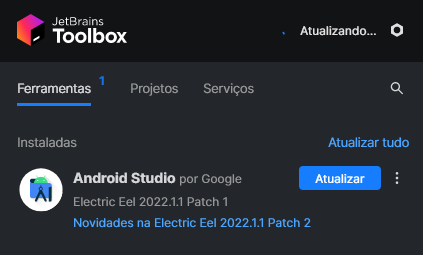
\includegraphics{images/toolbox.png}
  \caption{\textit{JetBrains Toolbox App}}
  % \acsfont{Fonte: Autoria própria}
  \label{fig:toolbox}
\end{figure}

Após instalado, é necessário abrir o Android Studio, fazer sua configuração inicial e configurar mais alguns passos, dentre eles, fazer a instalação de um emulador Android para utilizar no desenvolvimento, caso não queira utilizar um dispositivo físico, veja a seguir:
\begin{enumerate}
   \item Habilitar a "aceleração de VM" em sua máquina Windows;
   \item Na tela inicial do Android Studio, clique no ícone \textit{AVD Manager} e selecione \textit{Create Virtual Device…};
   \item Escolha uma definição de dispositivo e selecione "Avançar";
   \item Selecione uma ou mais imagens do sistema para as versões do Android que deseja emular e selecione Avançar. Uma imagem x86 ou x86\_64 é recomendada;
   \item Na aba de Performance do emulador, selecione Hardware - GLES 2.0 para habilitar a aceleração de hardware;
   \item Verifique se tudo está correto e selecione "Concluir";
   \item Por fim, basta executar o emulador e ele iniciará;
 \end{enumerate}

 Outro passo imprescindível é ativar as ferramentas \ac{sdk} necessárias para a compilação do projeto Flutter em um arquivo executável \textsc{.apk} para o Android, basta seguir este passo a passo:
 
 \begin{enumerate}
   \item Na tela inicial do Android Studio, clicar em \textit{File > Settings > Appearance \& Behavior > System Settings > \textit{Plugins}};
   \item Na aba \textit{Marketplace}, busque e instale os \textit{plugins} "Dart" e "Flutter";
   \item Nesta mesma tela, no menu lateral, clique em \textit{Appearance \& Behavior > System Settings > Android \ac{sdk}};
   \item Na aba \textit{\ac{sdk} Tools}, verifique se existem versões instaladas para \textit{Android SDK Build-Tools 34-rc2}, caso não, instale a correspondente à versão do Android escolhida na criação do emulador ou a do seu dispositivo físico;
   \item Ainda na aba \textit{\ac{sdk} Tools}, verifique se existe pelo menos uma versão instalada para \textit{Android SDK Command-line Tools}, caso contrário, instale a última versão disponível;
   \item Ainda na aba \textit{\ac{sdk} Tools}, verifique se o \textit{Android SDK Platform-Tools} está instalado, caso contrário, instale;
   \item Opcional: Ainda na aba \textit{\ac{sdk} Tools}, verifique se o \textit{Intel x86 Emulator Accelerator (HAXM installer)} está instalado, caso contrário, instale (esta ferramenta melhora a performance do emulador caso seu sistema suporte);
 \end{enumerate}
 
\subsection{Instalação do VSCode}\label{ssec:instalacao_vscode}
É possível seguir com o desenvolvimento no Android Studio, porém ele é um software que exige bastante processamento, o que pode "pesar" no sistema, portanto, existe a possibilidade de utilizar o VSCode\footnote{\label{vscode}VSCode: \url{https://code.visualstudio.com/}} para seguir como software padrão de desenvolvimento, além disso, no VSCode é possível instalar uma grande quantidade de pacotes desenvolvidos pela comunidade que agilizam o desenvolvimento, para utilizar o VSCode basta instalá-lo pela loja do \ac{so}, no caso do Windows, a \textit{Microsoft Store} ou pelo site oficial\footref{vscode}. 

Após instalado e feito a configuração inicial, basta buscar e instalar os \textit{plugins} "Dart" e "Flutter", outros de sua preferência também podem ser instalados. Por fim, basta criar (seguindo o tutorial oficial\footnote{\label{create_app}Escreva seu primeiro aplicativo Flutter: \url{https://docs.flutter.dev/get-started/codelab}}) ou abrir um projeto Flutter já existente e começar a editar seu código.

\subsection{Ferramentas e bibliotecas de suporte}\label{ssec:ferramentas}
% Descrever as ferramentas e bibliotecas de suporte utilizadas no desenvolvimento, tais como o Visual Studio Code, o Dart DevTools, o Flutter DevTools e as bibliotecas de terceiros que podem ser utilizadas para ajudar no desenvolvimento da aplicação.
Além dos \acp{ide}, outras ferramentas foram utilizadas para o desenvolvimento do sistema, nesta subseção abordo brevemente cada uma e sua aplicação.
\subsubsection{Flutter DevTools}\label{sssec:flutter_devtools}
O DevTools\footnote{\label{dev_tools}DevTools: \url{https://docs.flutter.dev/development/tools/devtools/overview}} é um conjunto de ferramentas de desempenho e depuração para Dart e Flutter, vem integrado na instalação do Flutter e executa automaticamente na inicialização de \textit{debugging}, suas principais funções são:

 \begin{enumerate}
   \item Inspecionamento do layout da interface do usuário e o estado de um aplicativo Flutter;
   \item Diagnóstico de problemas de instabilidade no desempenho da interface do usuário em um aplicativo Flutter;
   \item Visualização de informações gerais de \textit{log} e diagnóstico sobre um aplicativo de linha de comando Flutter ou Dart em execução;
   % \item Entre outras funcionalidades;
 \end{enumerate}

\subsubsection{Postman}\label{sssec:postman}
O Postman\footnote{\label{postman}Postman: \url{https://www.postman.com/}} é uma ferramenta de teste de \ac{api} que permite aos desenvolvedores testar, documentar e compartilhar suas APIs. Com o Postman, é possível enviar solicitações \ac{http}, verificar as respostas da \ac{api}, criar scripts de teste automatizados e compartilhar coleções de solicitações com outras pessoas. A ferramenta é amplamente utilizada no desenvolvimento de software e pode ser integrada a outras ferramentas, como o Swagger\footnote{\label{swagger}Swagger: \url{https://swagger.io/}}, para tornar o processo de teste e documentação de \acp{api} mais eficiente.

\subsubsection{\textit{Packages} do pub.dev}\label{sssec:pubdev}
Os \textit{packages} do pub.dev\footnote{\label{pubdev}pub.dev: \url{https://pub.dev/}} são bibliotecas de código-fonte aberto, desenvolvidas por membros da comunidade Flutter, que podem ser utilizadas para implementar recursos em \acp{app} Flutter. Essas bibliotecas fornecem funcionalidades prontas para uso, como a integração com \acp{api}, manipulação de imagens, gerenciamento de estado, entre outras. 

Ao utilizar um \textit{package} do pub.dev, os desenvolvedores podem economizar tempo e esforço na implementação de funcionalidades comuns, além de poderem se beneficiar de contribuições e correções de \textit{bugs} feitas pela comunidade. Os \textit{packages} podem ser facilmente adicionados ao projeto por meio do arquivo \textsc{pubspec.yaml} e instalados por meio do comando \inlinecode{flutter pub get}.

% \subsection{Integrações}\label{ssec:integracoes}
% Abordar integração com a API do backend, outros serviços e plataformas
% % é importante descrever os passos necessários para configurar essas integrações, tais como a integração com bancos de dados, serviços de autenticação, serviços de notificação e outros.

% \subsection{Gerenciamento de dependências}\label{ssec:gerenciamento_dependencias}
% Gerenciamento de dependências: É importante descrever como foram gerenciadas as dependências da aplicação, incluindo as ferramentas utilizadas para gerenciamento de pacotes e bibliotecas, tais como o Pub e o Flutter Packages.

% \subsection{Fluxo de trabalho de desenvolvimento}\label{ssec:fluxo_desenvolvimento}
% Descrever o fluxo de trabalho utilizado durante o desenvolvimento da aplicação, incluindo a metodologia de desenvolvimento adotada, as ferramentas utilizadas para controle de versão e colaboração entre os desenvolvedores, e os processos de testes e validação da aplicação.


% \section{Armazenamento e fornecimento de informações}
% \lipsum[1]

\section{Sprints}\label{sec:sprint}
Como foi explicado na seção de \nameref{ssec:metodologias_ageis}, o projeto seguiu duas metodologias que guiaram a criação do \ac{app}, o Scrum e o Kanban, muitas vezes referenciado por profissionais como "Scranban" ou algo semelhante, somente um nome genérico que aponte a junção dessas duas metodologias, portanto, o desenvolvimento do projeto foi dividido em sprints, houve um acordo entre a equipe sobre a flexibilidade das mesmas, visto que todos os envolvidos teriam que alinhar seus horários para a conclusão do projeto, ponderando entre sua vida acadêmica e profissional, o que acarretou em uma maior duração, mas não em menor desempenho ou qualidade, assim, impossibilitando manter uma sprint fixa de 2 a 4 semanas como sugerido pelo \textit{framework} Scrum. 

Como o uso do Kanban também estava presente, para a sprint ser iniciada havia um requisito: as atividades deveriam ser puxadas da coluna "TODO" na ordem de sua prioridade, portanto, com base na importância dos mesmos, tendo como foco a conclusão de um \ac{mvp}. Logo que o \ac{app} atingiu os requisitos mínimos esperados, foi gerado uma versão \textit{beta} e liberada para os usuários internos testarem, a fim de obter alguns \textit{feedbacks}.

Abaixo é possível ver uma demonstração do quadro de atividades do projeto Enzitech no Github Project\footnote{\label{githubproject}Github Project: \url{https://docs.github.com/en/issues/planning-and-tracking-with-projects/learning-about-projects/about-projects}}, plataforma utilizada como quadro adaptável, que se integra às \textit{issues} e solicitações de \textit{pull} no GitHub para ajudar no planejamento e acompanhar o projeto com eficiência.

\begin{figure}[H]
\centering
  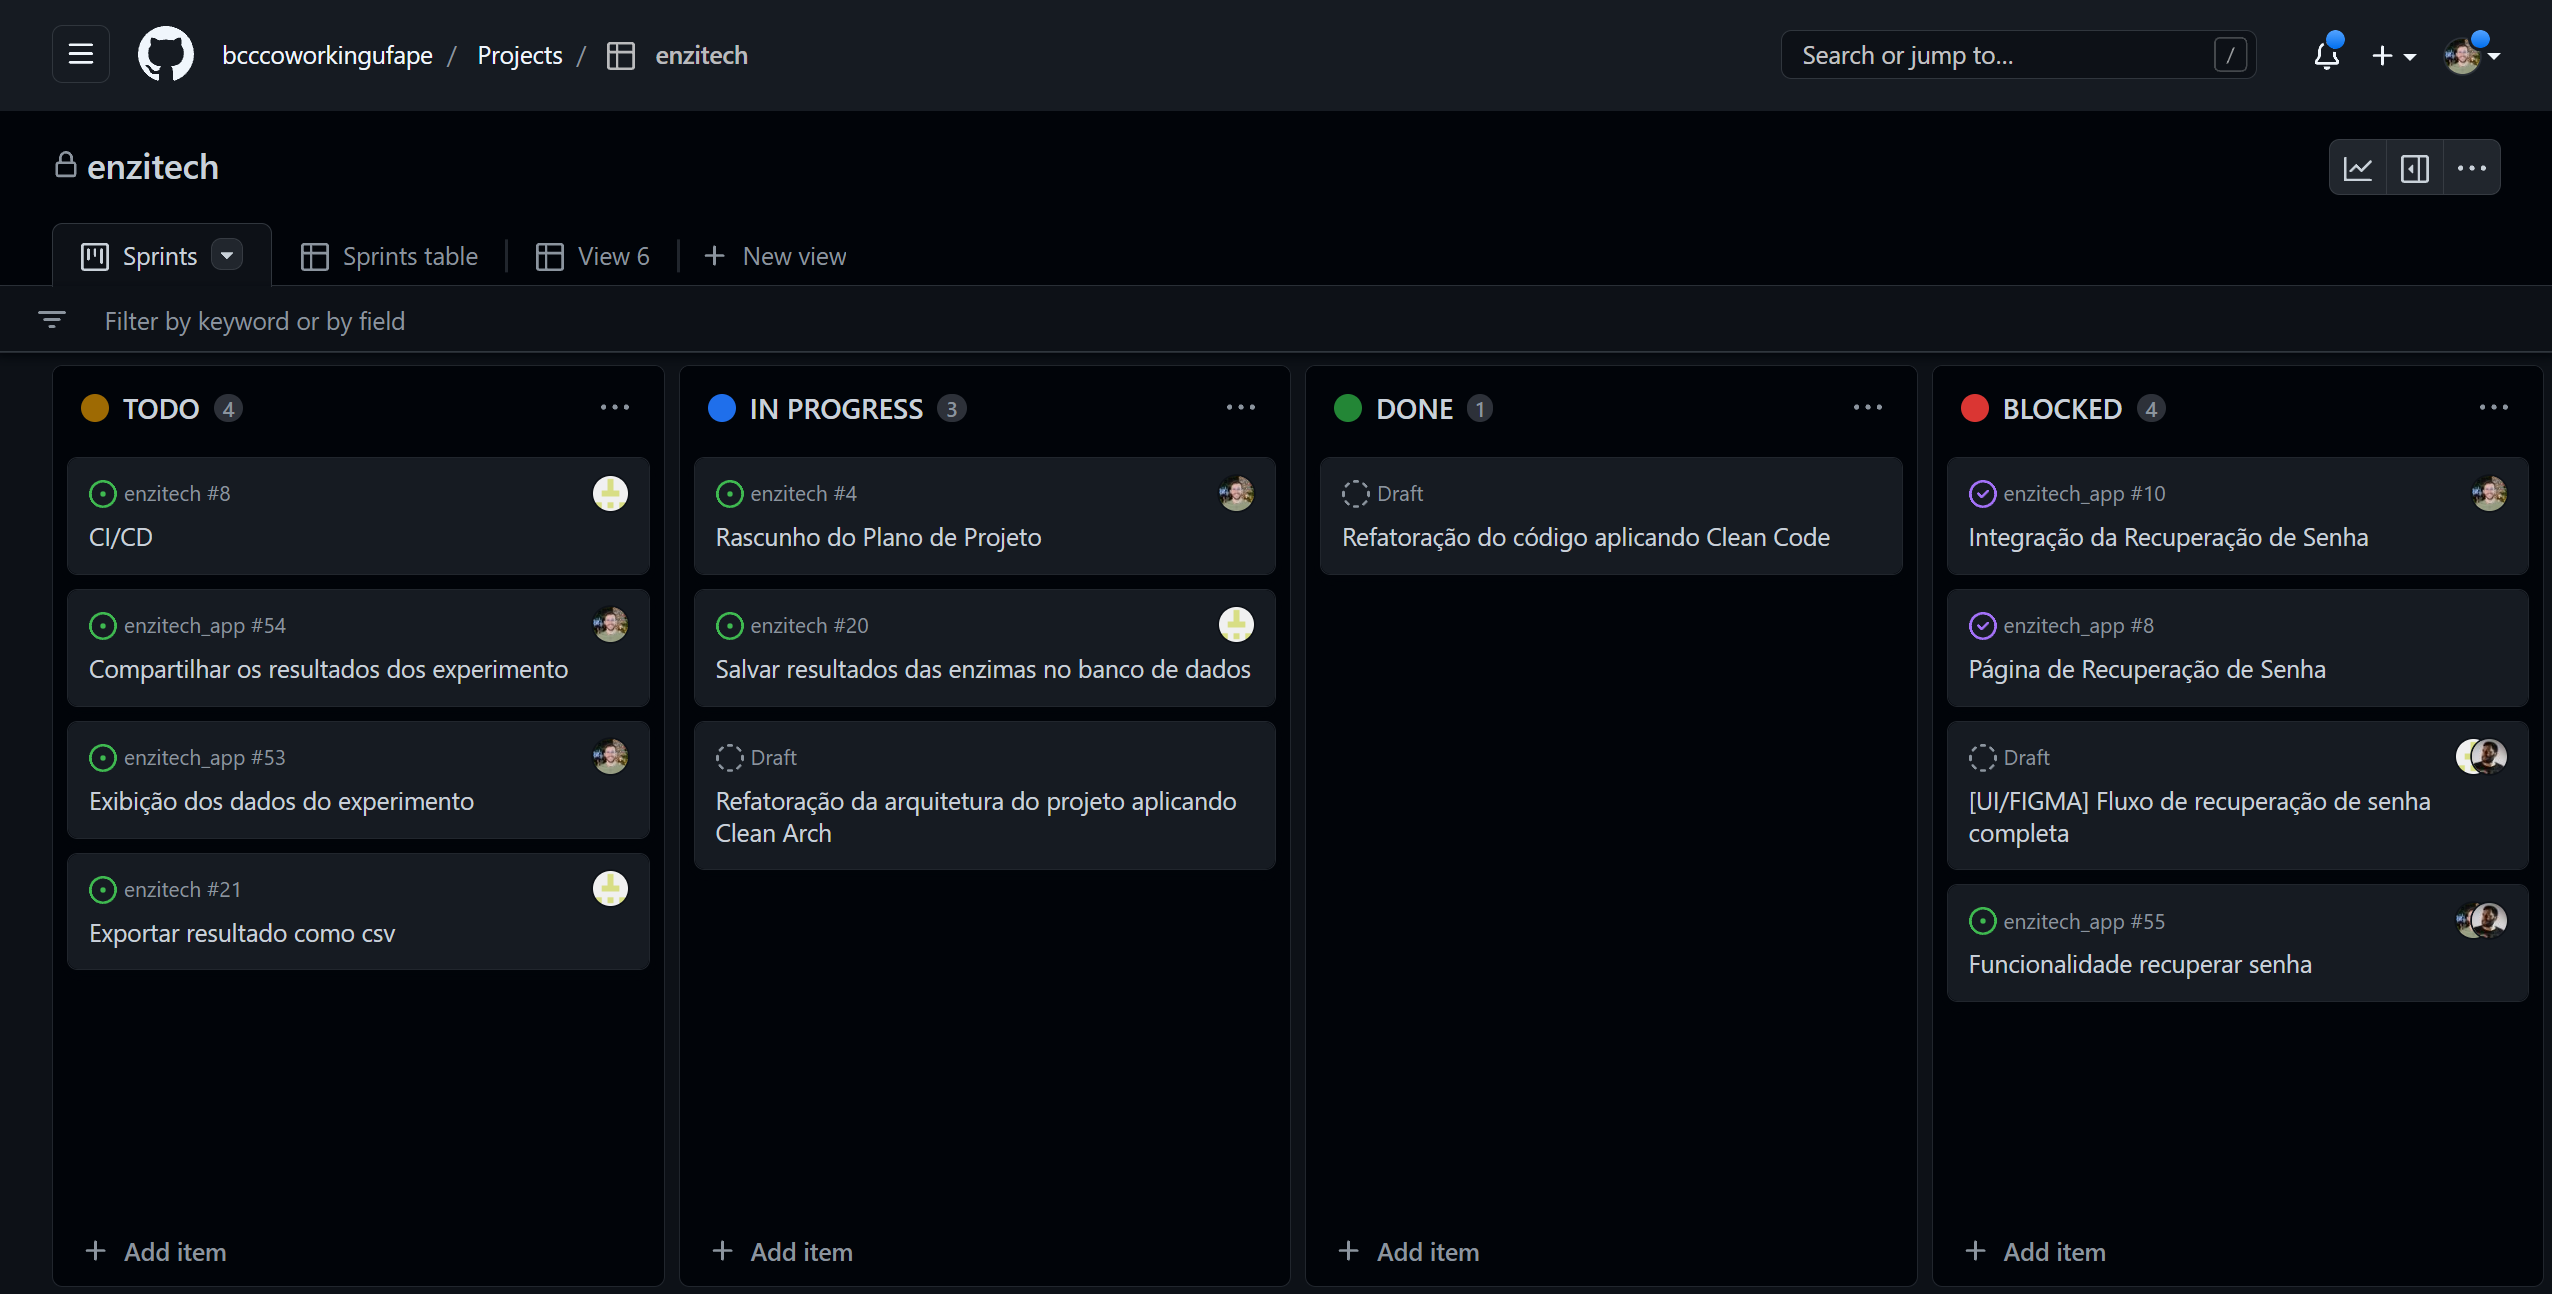
\includegraphics[width=\columnwidth]{images/quadro_projeto_github.png}
  \caption{Quadro de atividades do Enzitech no Github Project\footref{githubproject}}
  \acsfont{Fonte: Github}
  \label{fig:quadro_projeto_github}
\end{figure}

Outro dado interessante para a gestão ágil do projeto é o gráfico de eficiência e bloqueios, algo que também é disponibilizado no Github Project\footref{githubproject}, onde é possível ver o progresso do que está sendo feito para a conclusão do projeto, o fluxo de desenvolvimento e as mudanças de escopo ao longo do tempo. Sendo possível identificar gargalos e problemas que impedem o progresso da equipe. Abaixo está um exemplo do gráfico do projeto.

\begin{figure}[H]
\centering
  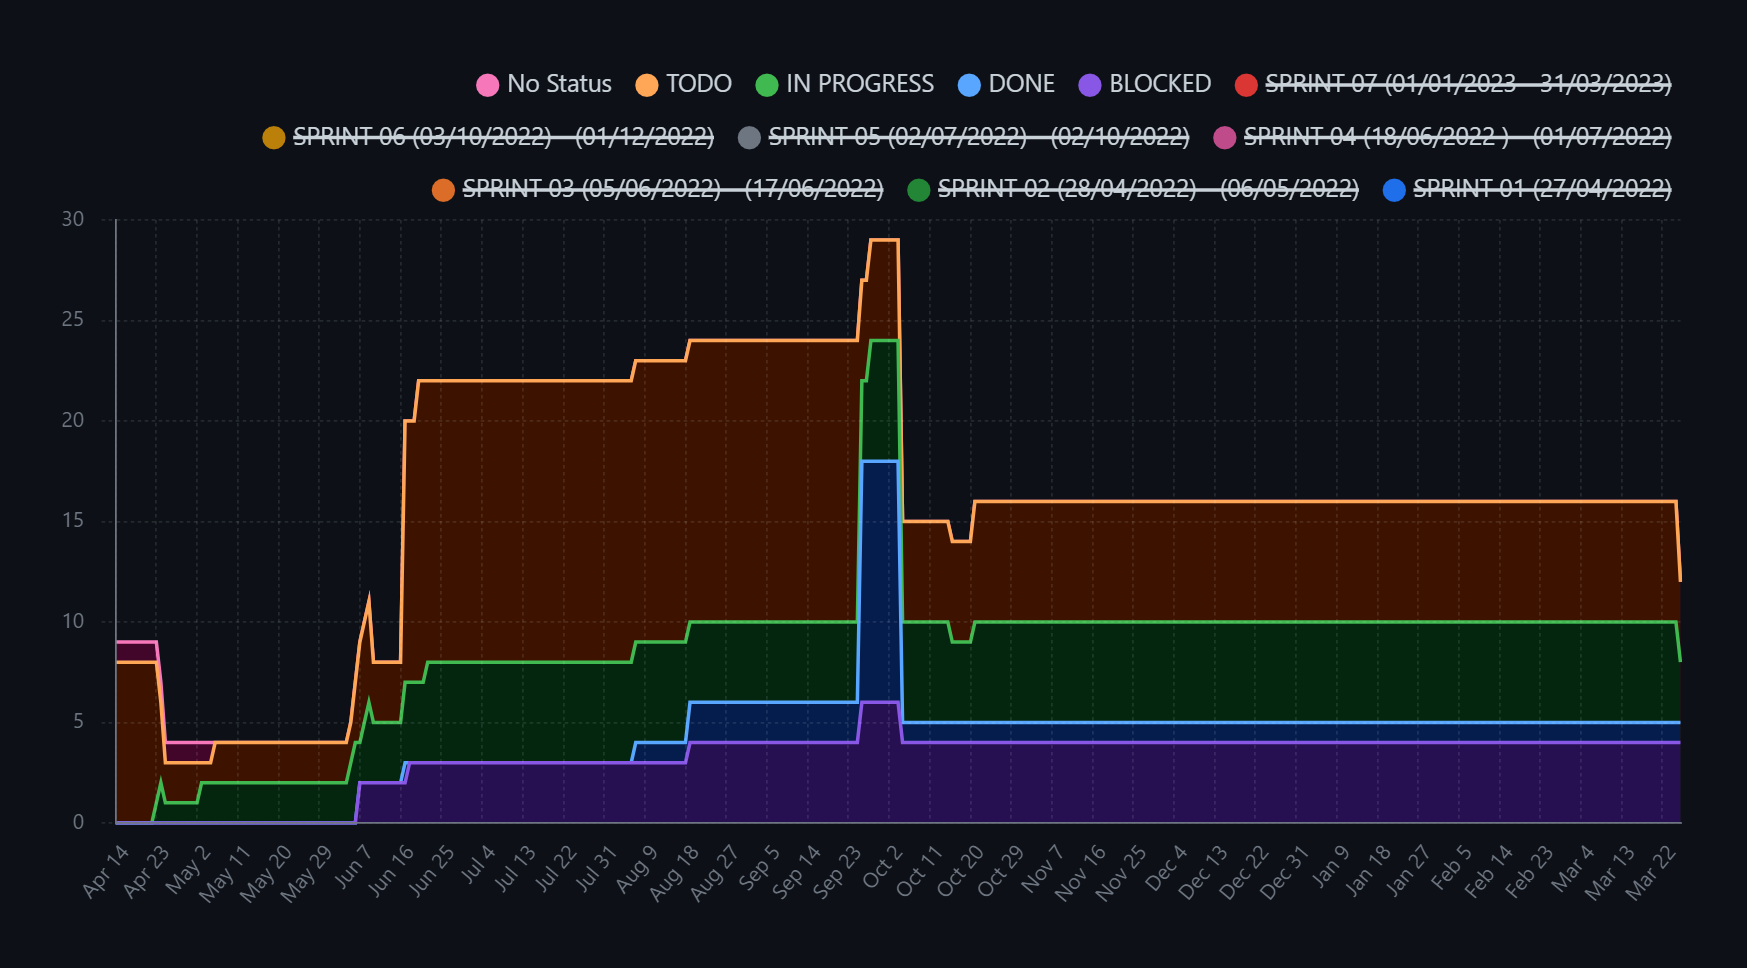
\includegraphics[width=\columnwidth]{images/grafico_projeto_github.png}
  \caption{Gráfico de \textit{Burn Up} das atividades do Enzitech no Github Project\footref{githubproject}}
  \acsfont{Fonte: Github}
  \label{fig:grafico_projeto_github}
\end{figure}

A seguir serão explicadas brevemente o planejamento, desenvolvimento e resultados obtidos em cada sprint.

\subsection{Sprint 1}\label{ssec:sprint1}

% \subsubsection{Planejamento}\label{sssec:planejamento1}
Para a primeira sprint, foi planejado o estudo da última versão do protótipo, o desenvolvimento da identidade visual do \ac{app}, incluindo seu ícone/logotipo, o \textit{back-end} tratou de desenvolver o \ac{crud} de usuários, assim como a documentação da \ac{api} que seria acessada pelo \textit{front-end(mobile)}, além disso, houve a configuração inicial dos bancos de dados e servidores para os ambientes de teste e desenvolvimento.

Simultaneamente, houve um estudo para decidir qual arquitetura seria adotada no \ac{app}, seu sistema de gerenciamento de estado e outros detalhes técnicos, como a criação do arquivo de \textit{design-system} para o \ac{app}. 

Nesta primeira sprint não houveram muitos impedimentos, e tudo fluiu dentro do esperado, levando em consideração que o projeto estava sendo criado e configurado ainda dentro deste período.
% \subsubsection{Desenvolvimento}\label{sssec:desenvolvimento1}
% Como será explicada numa seção mais detalhada a frente, o padrão arquitetural escolhido foi o \ac{mvvm}
% \subsubsection{Resultados}\label{sssec:resultados1}

\subsection{Sprint 2}\label{ssec:sprint2}
Nesta segunda sprint foi iniciado o desenvolvimento da tela de \textit{home}, ainda sem integrações, somente para alinhar a estrutura do projeto com a arquitetura escolhida, o \ac{mvvm}, um padrão de arquitetura em \textit{software} que facilita a separação do desenvolvimento da interface gráfica do usuário do desenvolvimento da lógica de negócios ou lógica de \textit{back-end} (o \textit{model}), de modo que a \textit{view} não dependa de nenhuma plataforma de modelo específica.

\begin{figure}[H]
\centering
  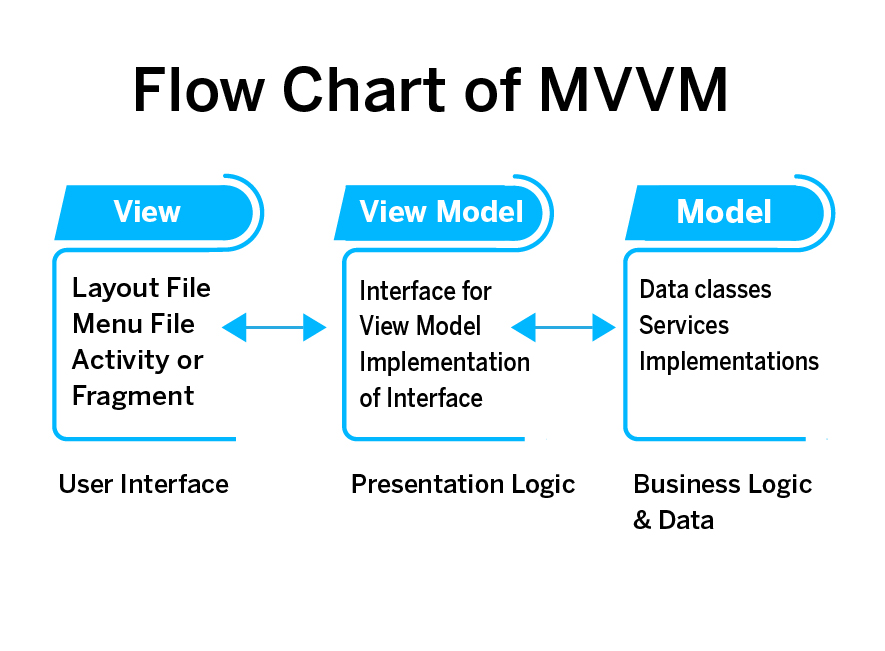
\includegraphics[width=\columnwidth/2]{images/MVVM-architecture.jpg}
  \caption{Descrição do padrão \ac{mvvm}}
  \acsfont{Fonte: \cite{appventurez}}
  \label{fig:MVVM-architecture}
\end{figure}

Além disso, foi desenvolvido a classe para requisições \ac{http} no \ac{app}, como também, mais telas foram desenhadas no protótipo de alta fidelidade. Ao fim, foi possível ter uma primeira versão executável do projeto, o qual já estava apto a se conectar à \textit{Web} e fazer requisições na \ac{api} que estava sendo desenvolvida em paralelo. 

\subsection{Sprint 3}\label{ssec:sprint3}
Os objetivos da terceira sprint foram implementar as telas e realizar as integrações dos \textit{endpoints} desenvolvidos para a \ac{api}, portanto, como resultado, foram contempladas os seguintes requisitos funcionais:
\begin{itemize}
   \item RF01 - Cadastro de usuário;
   \item RF02 - \textit{Login};
   \item RF03 - Recuperação de senha;
   \item RF12 - Listagem de experimentos;
 \end{itemize}

Ademais, o desenvolvimento do protótipo seguiu avançando e correções no código e na estrutura do \ac{app} foram realizadas, atingindo a seguinte estrutura:
\begin{figure}[H]
\centering
  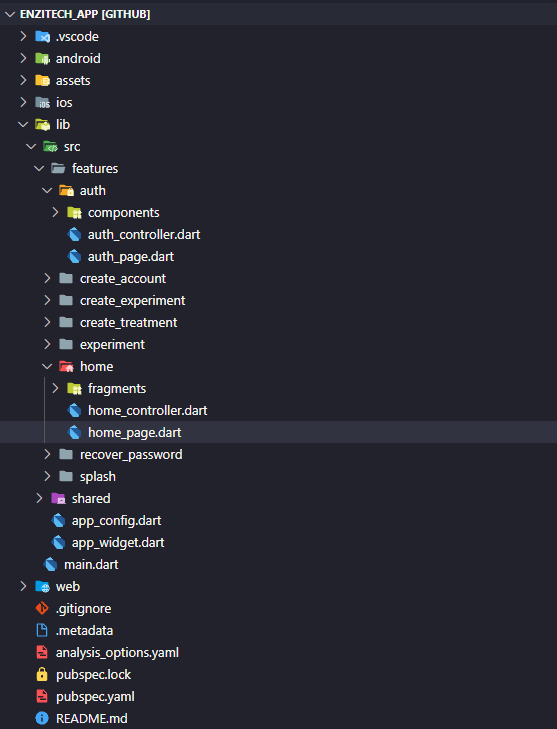
\includegraphics[width=\columnwidth/2]{images/app_sprint_3.png}
  \caption{Estrutura do projeto ao fim da terceira sprint}
  \acsfont{Fonte: Autoria própria}
  \label{fig:app_sprint_3}
\end{figure}

Outro ponto importante é que neste momento já foram adicionadas algumas dependências ao projeto que facilitaram o desenvolvimento, entre elas, é válido destacar as seguintes:
\begin{itemize}
   \item \textit{dio}: Biblioteca utilizada para realizar requisições \ac{http};
   \item \textit{provider}: Biblioteca utilizada para lidar com o gerenciamento de estado do \ac{app};
   \item \textit{shared\_preferences}: Biblioteca utilizada para armazenar dados simples de forma persistente no dispositivo;
 \end{itemize}

 Abaixo um trecho da \textit{view} de \textit{Home Page} desenvolvida até este ponto.

\begin{code}
\captionof{listing}{Home Page}
\label{code:dart-code}
\begin{minted}{dart}
// imports suprimidos

class HomePage extends StatefulWidget {
  const HomePage({Key? key}) : super(key: key);

  @override
  State<HomePage> createState() => _HomePageState();
}

class _HomePageState extends State<HomePage> {
  late final HomeController controller;
  late final ExperimentsController experimentsController;
  late final TreatmentsController treatmentsController;
  late final AccountController accountController;

  late List<Widget> _fragments;

  @override
  void initState() {
    super.initState();
    controller = context.read<HomeController>();
    experimentsController = context.read<ExperimentsController>();
    treatmentsController = context.read<TreatmentsController>();
    accountController = context.read<AccountController>();
    initFragements();
    if (mounted) {
      Future.delayed(Duration.zero, () async {
        await experimentsController.loadExperiments();
        await treatmentsController.loadTreatments();
        await accountController.loadAccount();
      });
      controller.addListener(() {
        if (controller.state == HomeState.error) {
          ScaffoldMessenger.of(context).showSnackBar(
            SnackBar(
              content: Text(controller.failure!.message),
            ),
          );
        }
      });
    }
  }

  initFragements() {
    _fragments = [
      ExperimentsPage(
        homeController: controller,
      ),
      TreatmentsPage(
        homeController: controller,
      ),
      AccountPage(
        homeController: controller,
      ),
    ];
  }

  Widget? get dealWithFloatingActionButton {
    if (controller.fragmentIndex == 0) {
      return FloatingActionButton.extended(
        onPressed: () {
          Navigator.pushNamed(
            context,
            RouteGenerator.createExperiment,
          );
        },
        label: Text(
          "Cadastrar\nexperimento",
          style: TextStyles.buttonBackground,
        ),
        icon: const Icon(
          PhosphorIcons.pencilLine,
          color: AppColors.white,
          size: 30,
        ),
      );
    }

    if (controller.fragmentIndex == 1) {
      return FloatingActionButton.extended(
        onPressed: () {
          Navigator.pushNamed(
            context,
            RouteGenerator.createTreatment,
          );
        },
        label: Text(
          "Cadastrar\ntratamento",
          style: TextStyles.buttonBackground,
        ),
        icon: const Icon(
          PhosphorIcons.pencilLine,
          color: AppColors.white,
          size: 30,
        ),
      );
    }

    return null;
  }

  @override
  Widget build(BuildContext context) {
    final controller = context.watch<HomeController>();

    return Scaffold(
      appBar: AppBar(
        title: SvgPicture.asset(
          'assets/images/logo.svg',
          fit: BoxFit.contain,
          alignment: Alignment.center,
        ),
      ),
      body: ChangeNotifierProvider(
        create: (BuildContext context) {},
        child: _fragments[controller.fragmentIndex],
      ),
      floatingActionButton: dealWithFloatingActionButton,
      bottomNavigationBar: BottomNavigationBar(
        items: const [
          BottomNavigationBarItem(
            icon: Icon(PhosphorIcons.flask),
            label: 'Experimentos',
          ),
          BottomNavigationBarItem(
            icon: Icon(PhosphorIcons.testTube),
            label: 'Tratamentos',
          ),
          BottomNavigationBarItem(
            icon: Icon(PhosphorIcons.userCircleGear),
            label: 'Conta',
          ),
        ],
        currentIndex: controller.fragmentIndex,
        selectedItemColor: AppColors.white,
        backgroundColor: AppColors.primary,
        onTap: (index) => controller.setFragmentIndex(index),
      ),
    );
  }
}
\end{minted}
\end{code}

Desta forma, adiantando a estrutura para as próximas \textit{features} a serem implementadas e obtendo como resultado um \ac{app} que já tomava o formato desejado, assim, entregando valor com a entrega da sprint.

\subsection{Sprint 4}\label{ssec:sprint4}
Nesta quarta sprint, os objetivos foram as implementações das telas e integrações dos \textit{endpoints} desenvolvidos que restavam, abrangindo os seguintes requisitos funcionais:
\begin{itemize}
   \item RF04 - Cadastro de tratamento;
   \item RF06 - Listagem de tratamentos;
   \item RF07 - Cadastro de enzima;
   \item RF09 - Listagem de enzimas;
   \item RF10 - Criação de experimento;
 \end{itemize}

 Neste ponto, o \ac{app} já possuía as principais \textit{features} para seguir com a parte de experimentos e cálculos, alguns testes foram realizados para verificar o fluxo de informações entre as telas e se tudo estava integrado corretamente, apesar do projeto ser desenvolvido para multiplataformas, vale salientar que inicialmente o \ac{app} só estará disponível para o sistema Android, visto que a publicação de \acp{app} neste sistema é muito mais simples e barata se comparada a \acp{app} para iOS, cuja licença para publicar \acp{app} na loja custa um valor considerável. Não é descartada a hipótese de lançar o \ac{app} para dispositivos iOS no futuro, contanto que exista demanda dos usuários para tal.

 O projeto necessitou de uma configuração no \textit{Firebase} \footnote{\label{firebase}\textit{Firebase}: \url{https://firebase.google.com/}} para o lançamento de versões internas para teste no \textit{App Distribution}, o que foi realizado aqui nesta sprint, com isso, foi possível escolher alguns usuários envolvidos no projeto para realizarem os testes, instalando o mesmo em seus dispositivos pessoais. 

 Abaixo, na \figref{fig:app_distribution}, uma demonstração do painel do \textit{App Distribution} para o \ac{app}, para utilizar este serviço foi preciso integrar o Firebase SDK no \ac{app} Flutter e configurar o processo de build para enviar o \textsc{.apk} ou \textsc{.aab} (versões compiladas para o Android) para o Firebase. Em seguida, foi necessário criar um grupo de testadores e conceder acesso ao \ac{app}.

Os testadores receberam um convite por e-mail com um link para fazer o download do \ac{app} e começar a testá-lo. No painel, é possível controlar quem tem acesso às versões do \ac{app}, permitindo que apenas usuários específicos o baixem e o testem, uma vez que ele tenha sido distribuído, é possível monitorar as métricas de uso e coletar feedback dos testadores, o que ajuda a melhorar o produto antes de lançá-lo oficialmente.

\begin{figure}[H]
\centering
  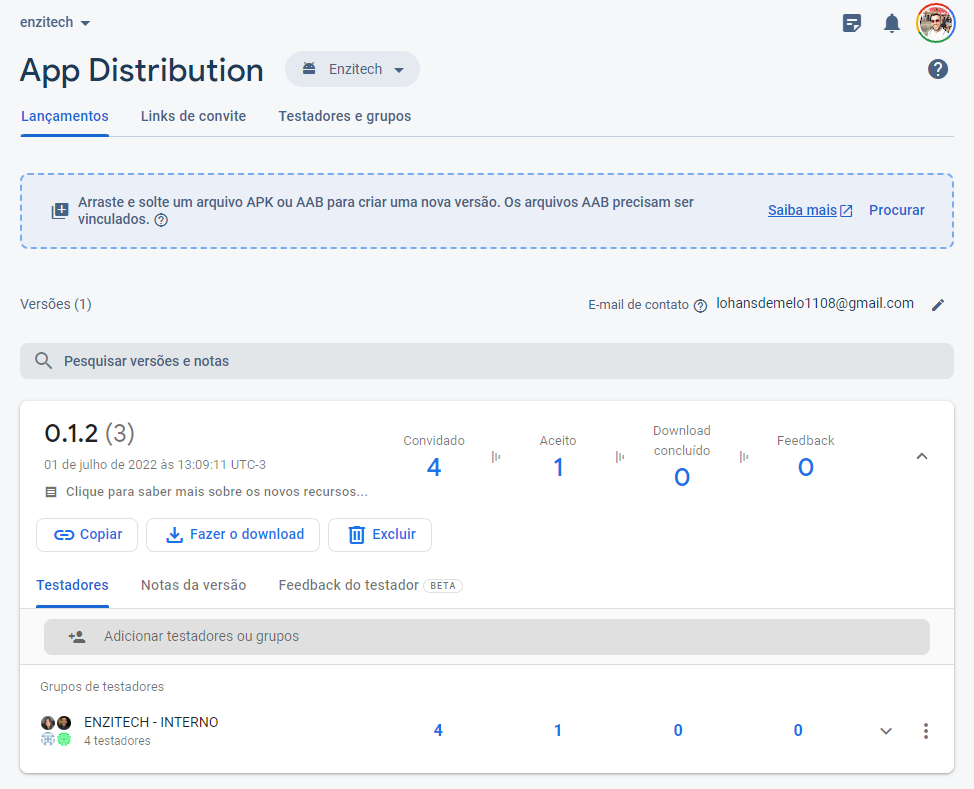
\includegraphics[width=\columnwidth]{images/app_distribution.png}
  \caption{Aba do \textit{Firebase App Distribution} do projeto Enzitech}
  \acsfont{Fonte: \textit{Firebase}\footref{firebase}}
  \label{fig:app_distribution}
\end{figure}
 
\subsection{Sprint 5}\label{ssec:sprint5}
Na quita sprint, o protótipo de alta fidelidade atingiu a maturidade que o projeto necessitava, desta forma o foco de desenvolvimento foi voltado para as implementações das \textit{features} de deletar as entidades que já eram possíveis serem criadas, desta forma, os seguintes requisitos funcionais foram concluídos:
\begin{itemize}
   \item RF05 - Deletar um tratamento;
   \item RF08 - Deletar uma enzima;
   \item RF11 - Deletar um experimento;
   \item RF13 - Utilizar filtros na listagem de experimentos;
 \end{itemize}

A RF13 foi iniciada nesta sprint, mas não foi concluída, pois a história foi dividida em duas \textit{spikes} — a definição de \textit{"Spike"} vem do \textit{Extreme Programming} e surgiu a partir da \textit{"Spike Solution"}, que é um programa ou protótipo funcional usado para explorar possíveis soluções para um problema específico — uma para o desenvolvimento de um \textit{switch} entre experimentos concluídos e em andamento e outra para o desenvolvimento do filtro por ordenação de características de um experimento, portanto, nessa, o \textit{switch} foi implementado, porém sem integrações com a \ac{api} ainda.

Nesta sprint mais requisitos foram concluídos, houveram vários ajustes e correções de \textit{bugs}, como os de fluxos após criação de um experimento, junto disso houveram alguns estudos para uma futura refatoração que será abordada na última sprint, foi notado que o escopo do projeto precisaria de uma arquitetura mais refinada, logo, este tempo foi reservado para estudo junto ao desenvolvimento.  
 
\subsection{Sprint 6}\label{ssec:sprint6}
Nesta sexta sprint, os seguintes requisitos funcionais foram atacados:
\begin{itemize}
   \item RF13 - Utilizar filtros na listagem de experimentos;
   \item RF14 - Visualizar detalhes de um experimento;
   \item RF15 - Inserção de dados para o cálculo enzimático no experimento;
 \end{itemize}

Na \figref{fig:filtros_sprint_6} é possível ver o \textit{dialog} desenvolvido para a escolha de filtros na listagem de experimentos, nele é possível escolher a ordenação por ordem crescente ou decrescente, assim como, é possível mudar a ordenação de acordo com o nome, descrição, repetições, progresso, data de criação ou data de modificação. Desta forma, finalizando o requisito funcional 13 por completo.
 
 \begin{figure}[H]
\centering
  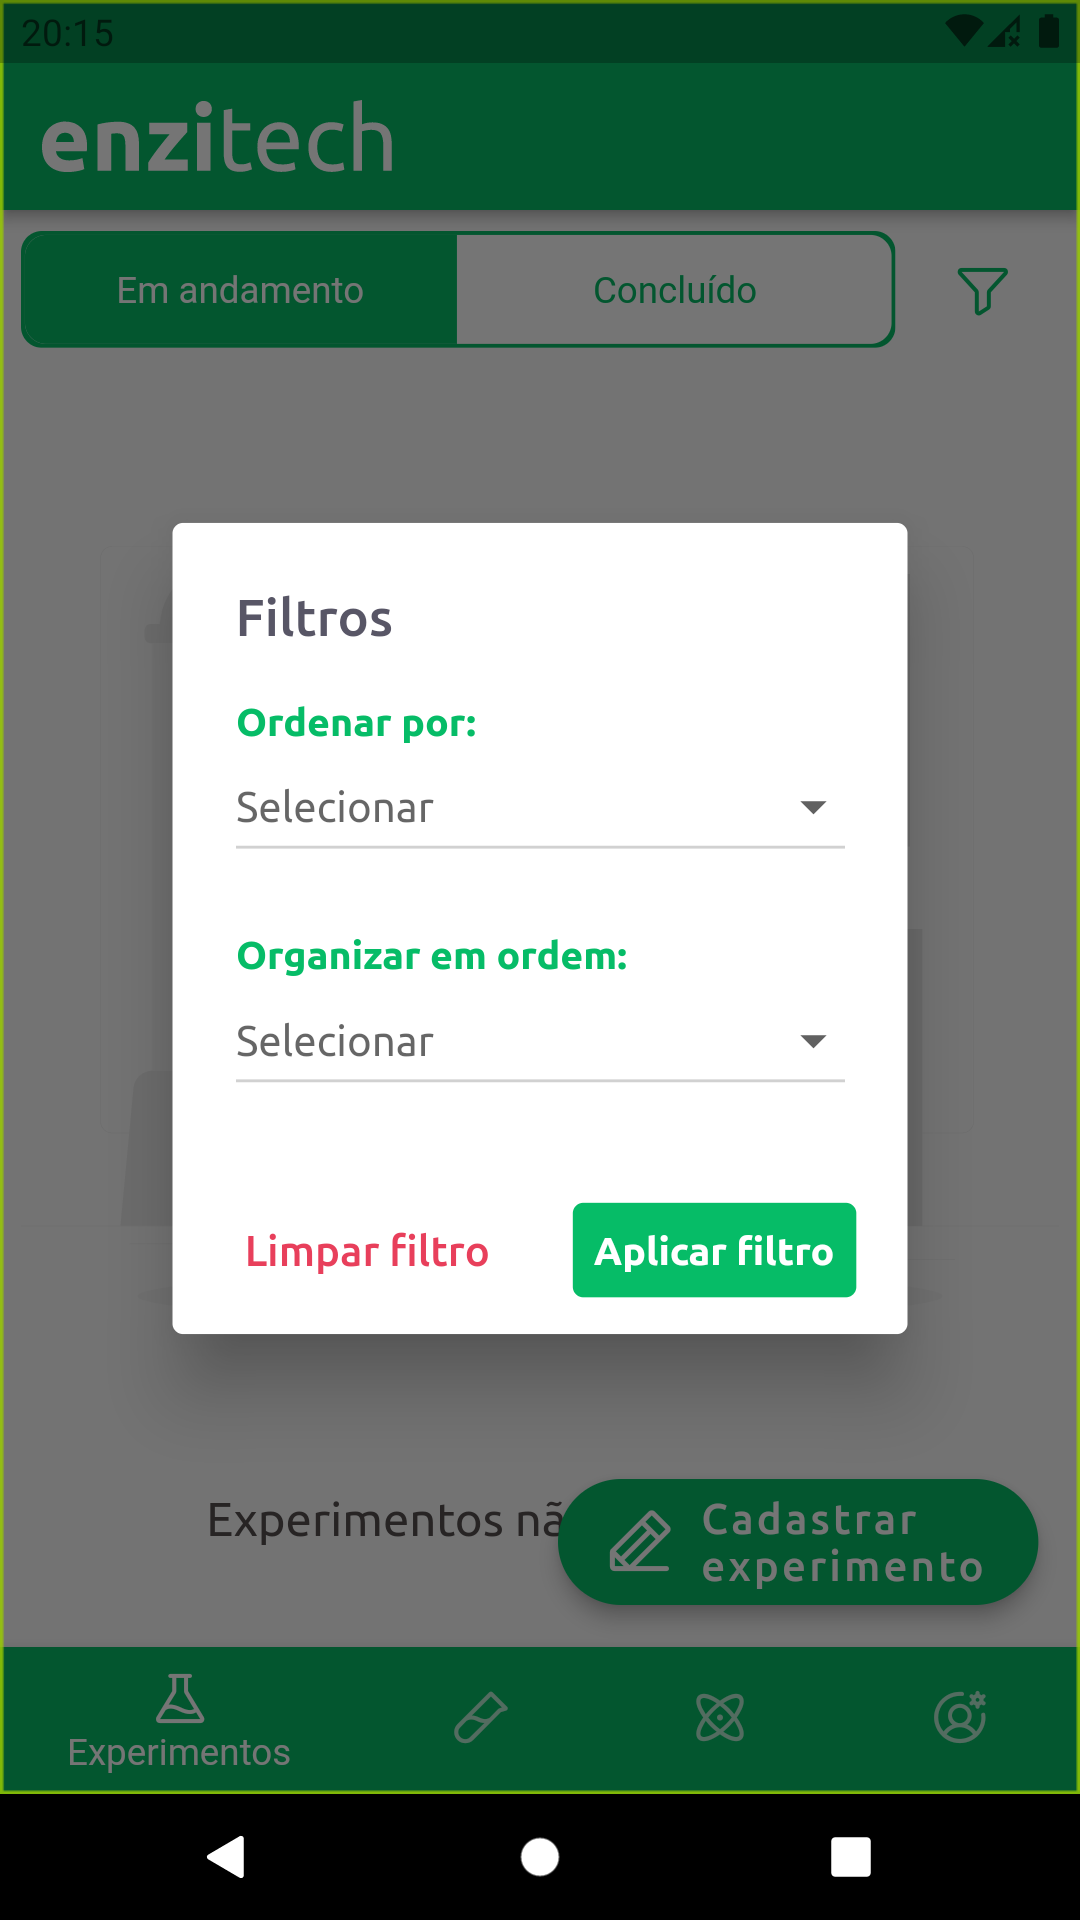
\includegraphics[width=\columnwidth/2]{images/filtros_sprint_6.png}
  \caption{Filtros de experimento do Enzitech}
  \acsfont{Fonte: Autoria própria}
  \label{fig:filtros_sprint_6}
\end{figure}

Aqui também foi desenvolvido todo o fluxo para visualização dos detalhes de um experimento, o que dá acesso às opções de inserir dados e visualizar os mesmos. Nesta sprint também foi aplicado um estudo de performance feito no \ac{app}, o qual até este momento só carregava os dados após a \textit{splashscreen} (tela antes da home/listagem de experimentos), o que não era o melhor cenário possível, então, após alguns artigos lidos e estudos de caso, a solução encontrada foi de fazer a primeira carga de informações do Enzitech ao \ac{app} ser aberto, ou seja, em sua inicialização, de forma assíncrona, onde, se preciso fosse, a tela de \textit{splashscreen} faria sua responsabilidade, que é de segurar a navegação do usuário até que todos os dados estejam preparados para o uso. 

Desta forma, houve um ganho de performance que diminuiu o tempo de carregamento do \ac{app}, trazendo uma sensação de maior fluidez.
\hfill \break
\begin{code}
\captionof{listing}{Trecho de código para realizar a checagem de autenticação e pré-carregamento dos dados}
\label{code:dart-code}
\begin{minted}{dart}
_checkAuth() async {
    Future.delayed(Duration.zero).then((_) async {
    String token = await getToken() ?? '';

    if (!mounted) return;

    if (token.isEmpty) {
        Navigator.pushReplacementNamed(context, RouteGenerator.auth);
    } else {
        await Provider.of<HomeViewmodel>(context, listen: false)
        .getContent()
        .then((value) =>
            Navigator.pushReplacementNamed(
                context, 
                RouteGenerator.home,
            ),
        );
      }
    });
  }
\end{minted}
\end{code}

Como podemos ver no Código Fonte \ref{code:dart-code} o sistema primeiro checa se há algum \textit{token} de autenticação guardado, caso negativo ele segue da \textit{splashscreen} de volta para a tela de \textit{login} para o usuário realizar a autenticação novamente, caso positivo a navegação segue, os dados são pré-carregados e logo após o usuário é levado para a tela inicial do Enzitech.

Além disso, foi implementado uma \textit{feature} para lidar com ações sensíveis, como a de exclusão de itens, desta forma, é possível ativar ou desativar nas configurações do \ac{app} um alerta de confirmação de exclusão de experimentos, tratamentos e enzimas, o qual, além deste passo de segurança implementado, oferece outra funcionalidade, independente desta anterior estar ativada ou não, que é a de desfazer ações destrutivas, ou seja, o usuário pode se arrepender da exclusão (ou tê-la feito por engano) e recuperar esta informação, assim, oferecendo um passo de segurança a mais para os dados, abaixo na \figref{fig:fluxo_exclusao} é possível ver sua aplicação em um tratamento.

\begin{figure}[H]

\centering
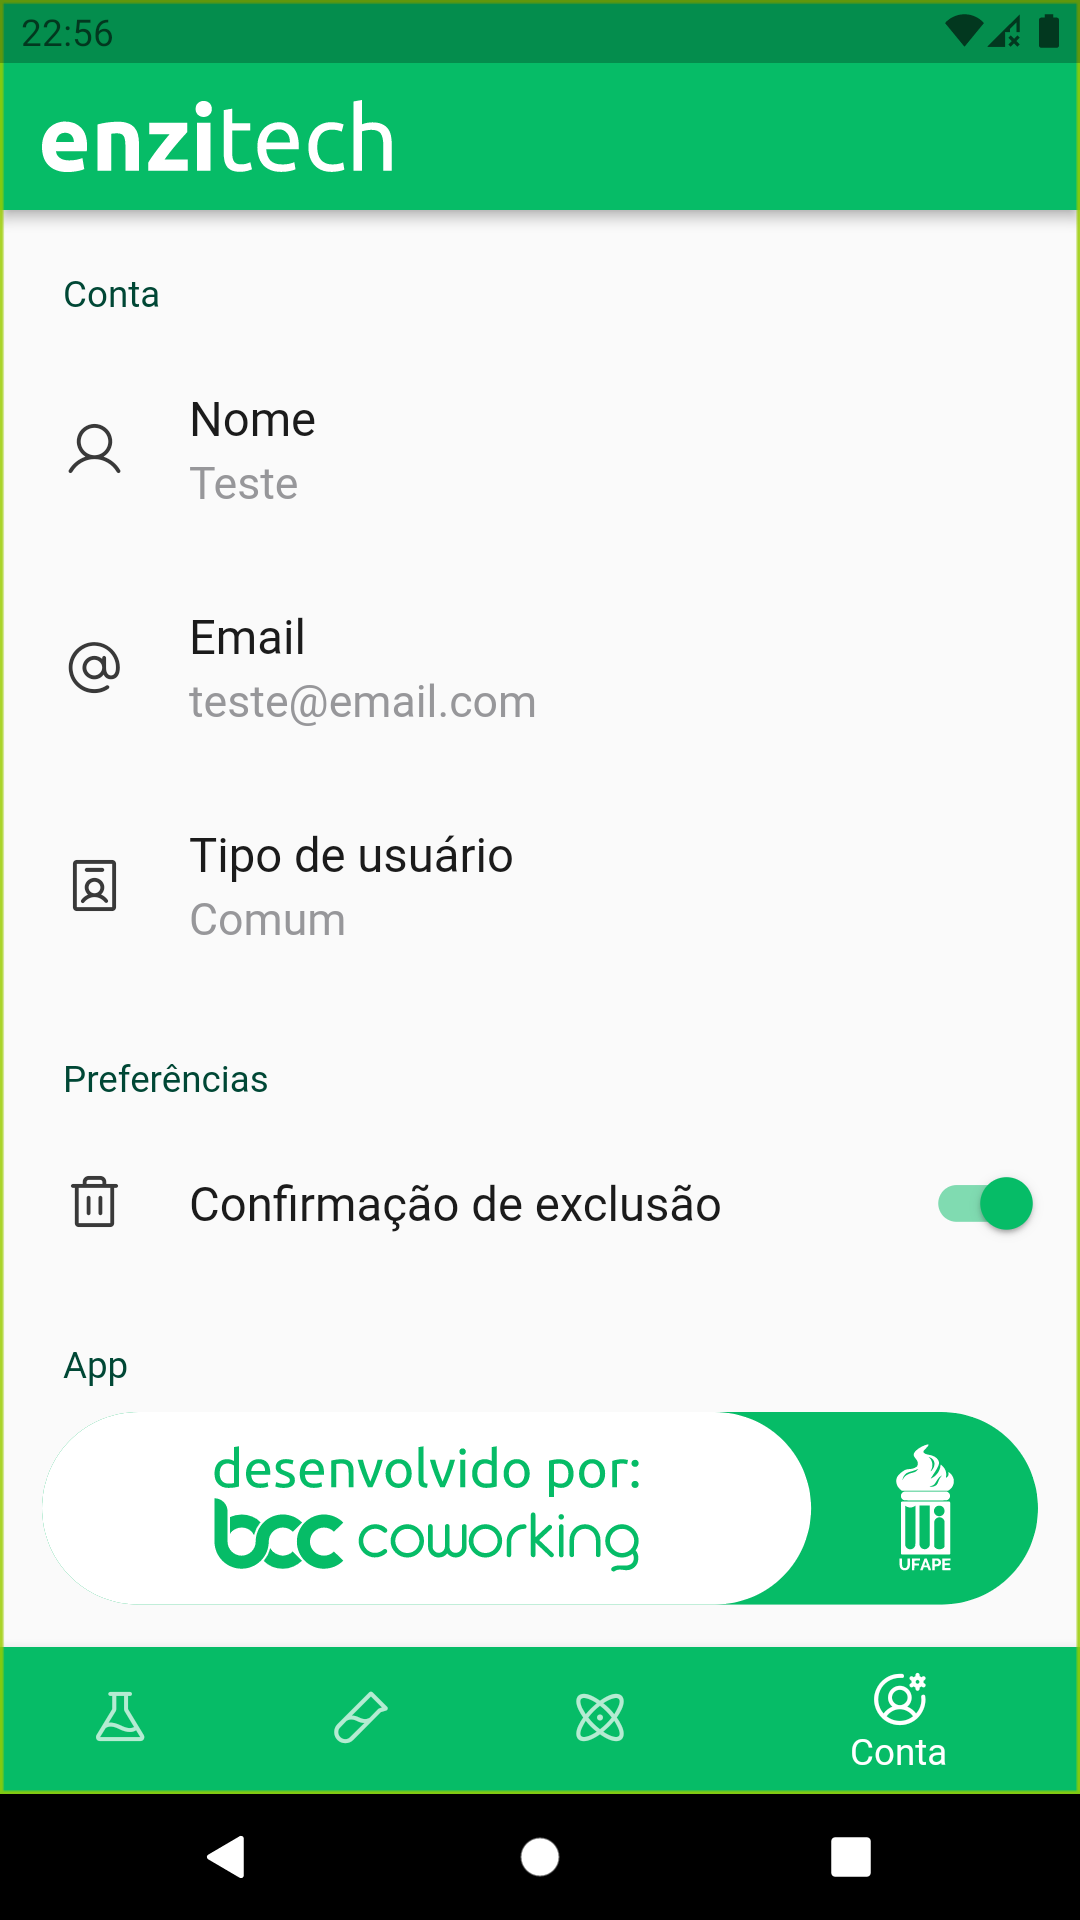
\includegraphics[width=.3\textwidth]{images/exclusao_1_sprint_6.png}\hfill
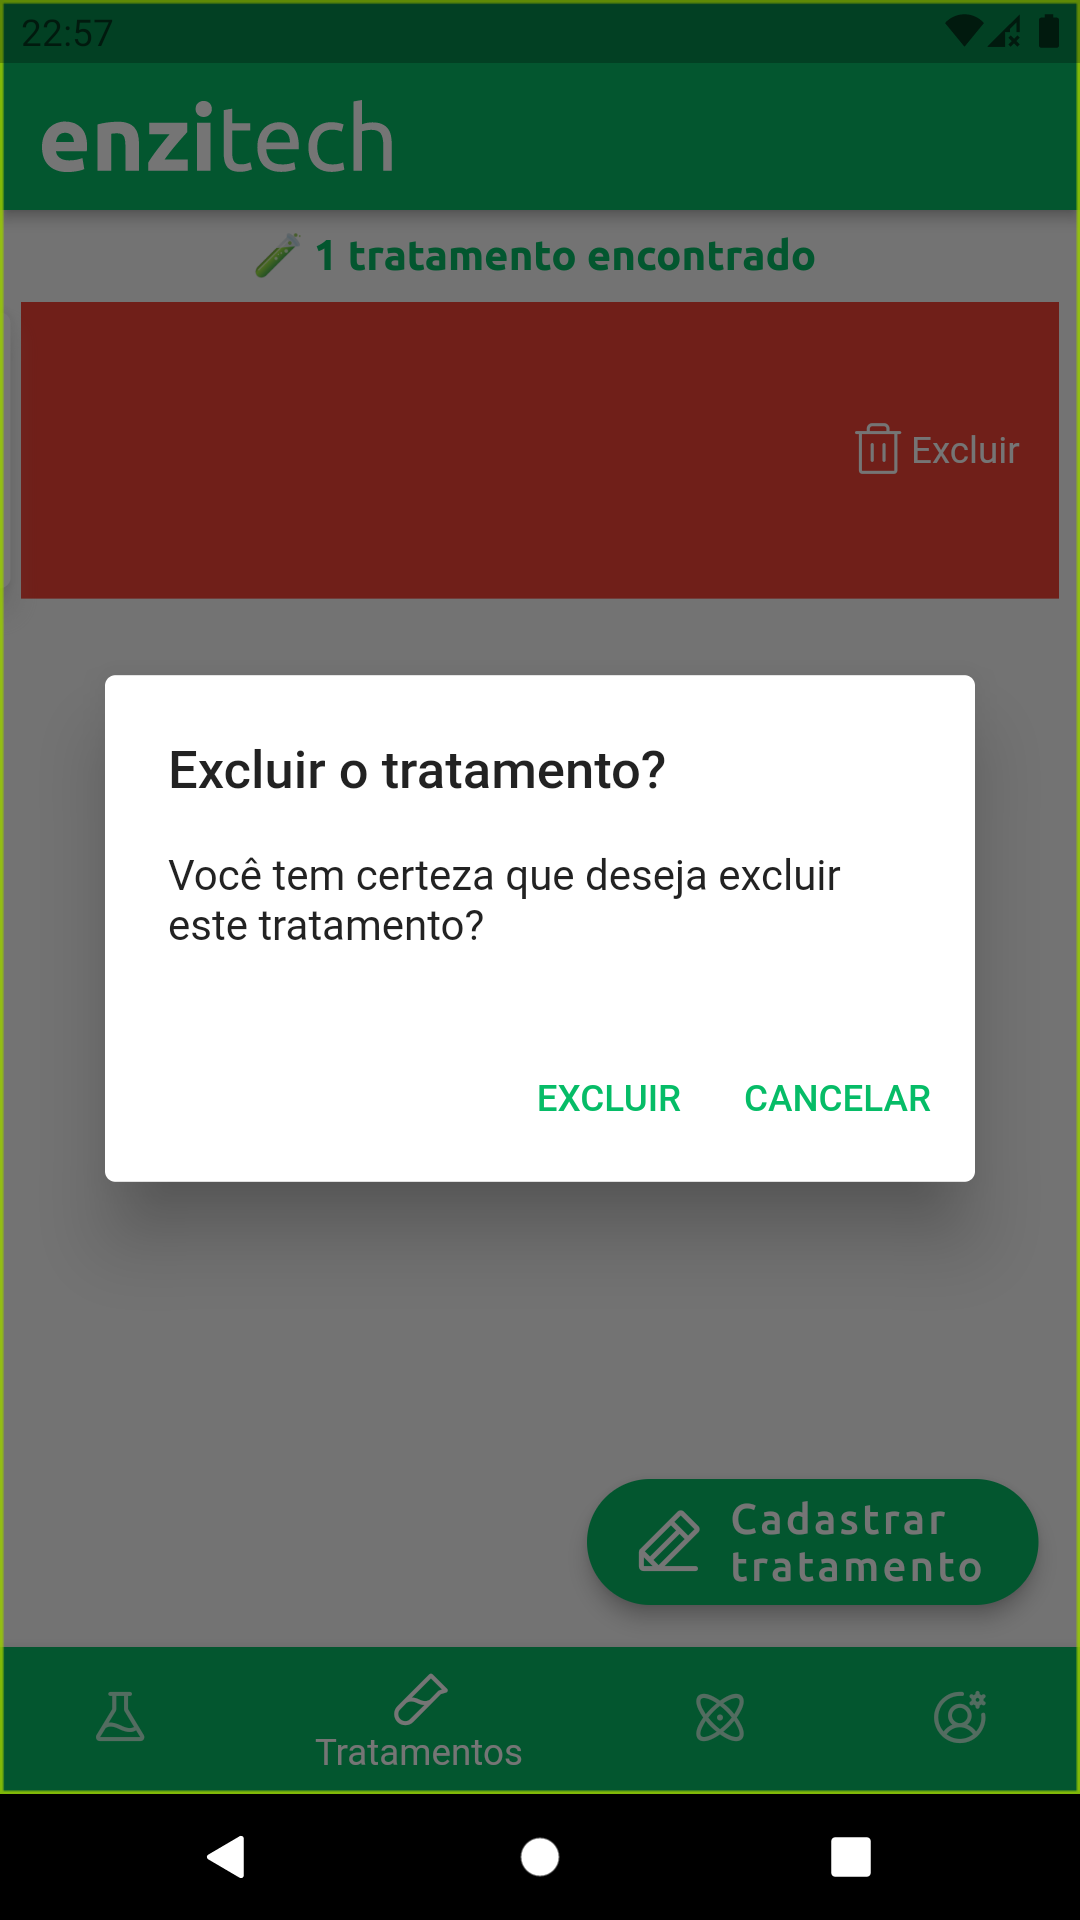
\includegraphics[width=.3\textwidth]{images/exclusao_2_sprint_6.png}\hfill
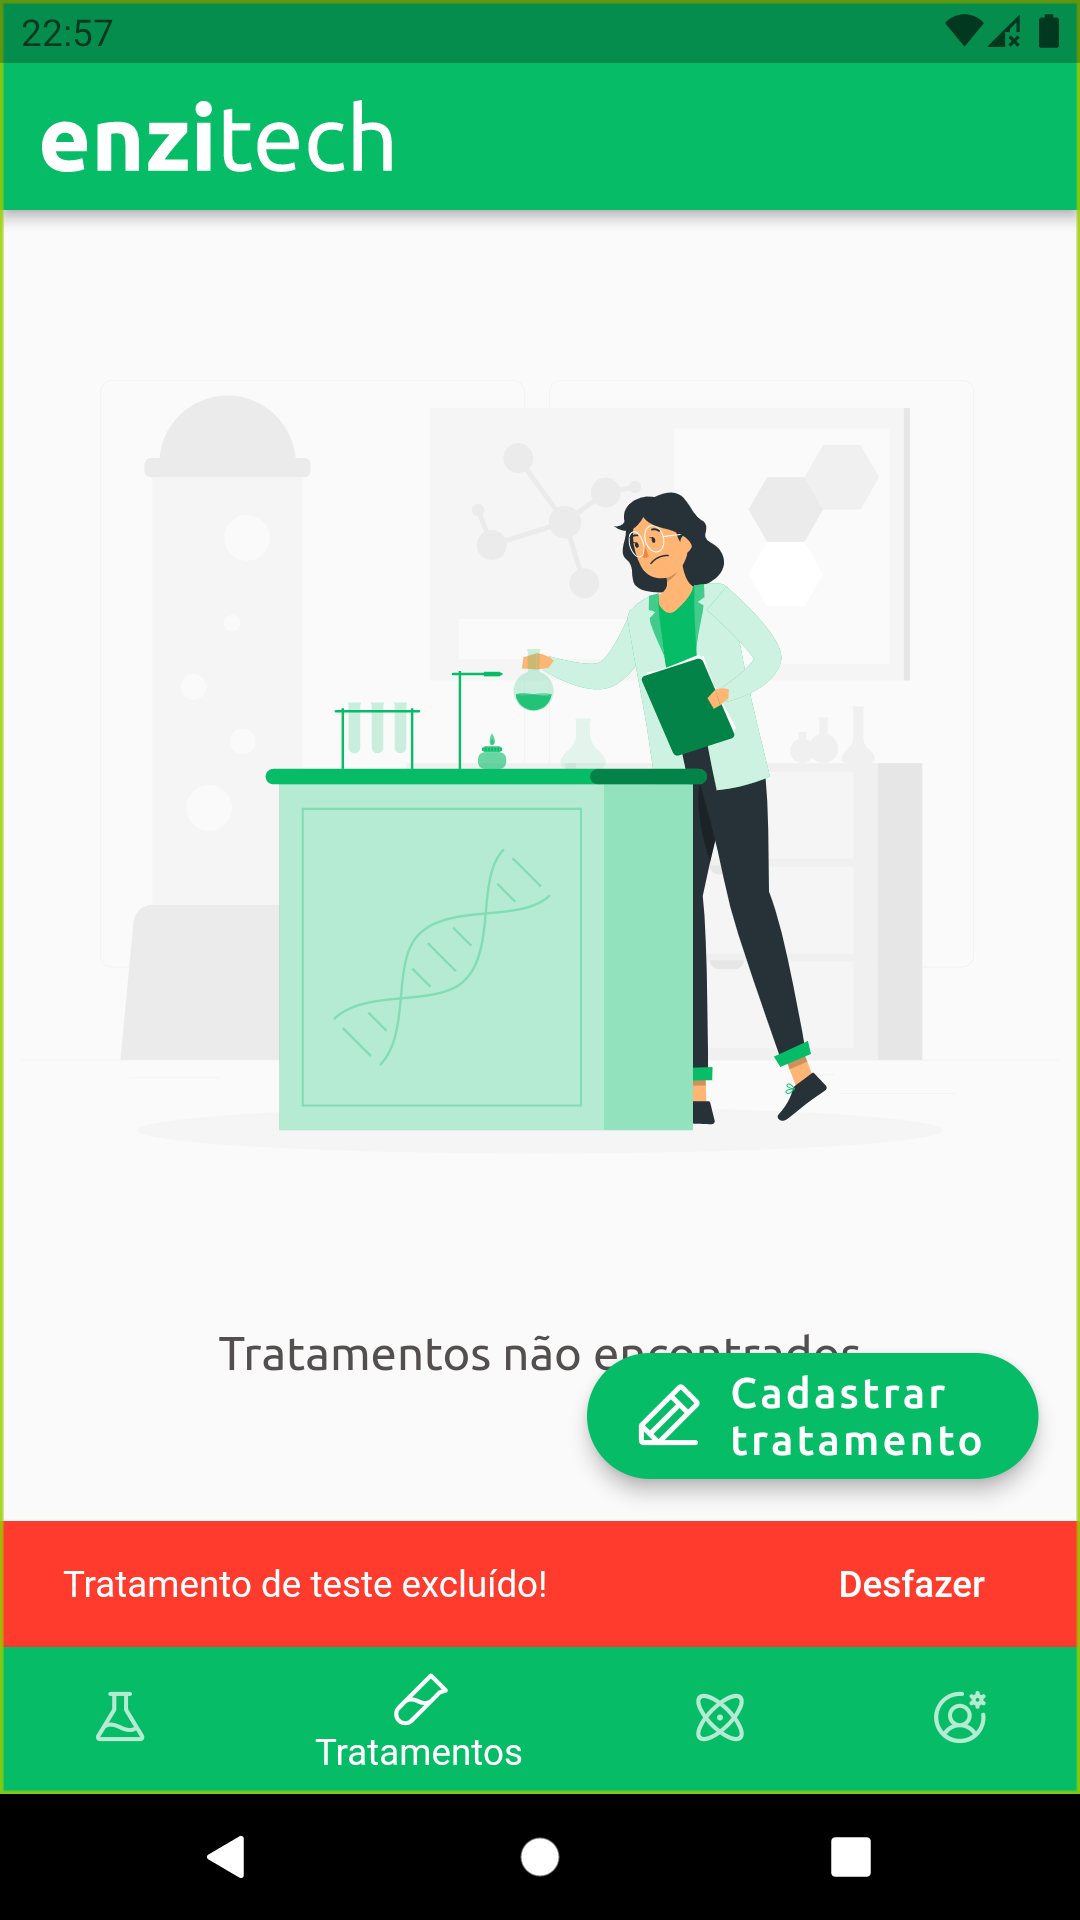
\includegraphics[width=.3\textwidth]{images/exclusao_3_sprint_6.png}

\caption{Fluxo de exclusão de um tratamento com a opção de confirmação de exclusão ativada}
\label{fig:fluxo_exclusao}

\end{figure}

\subsection{Sprint 7}\label{ssec:sprint7}
Na sétima e última sprint do projeto o projeto houve uma enorme refatoração de arquitetura, como comentado na subseção \ref{ssec:sprint4}, aqui, além dessa refatoração que não adiciona funcionalidades, mas garante a estabilidade do \ac{app} e permite que o mesmo possa receber novas funcionalidades de forma mais fácil e sem problemas, houve a conclusão dos requisitos funcionais restantes, são eles:
\begin{itemize}
   \item RF16 - Visualização de resultados discrepantes do cálculo enzimático antes de salvar no experimento;
   \item RF17 - Edição de resultados discrepantes do cálculo enzimático antes de salvar no experimento;
   \item RF18 - Opção de salvar os resultados do cálculo enzimático no experimento;
   \item RF19 - Visualização de todos os resultados e o progresso do experimento;
   \item RF20 - Exportação dos resultados do experimento;
 \end{itemize}

[EM DESENVOLVIMENTO até 31/03/23]

\section{Back-end}
O back-end do projeto foi desenvolvido pelo BCCCoworking, Laboratório de Pesquisa e Desenvolvimento, concebido no curso de Ciência da Computação da \ac{ufape}, sendo assim, nesta seção trago detalhes resumidos de sua implementação e como ele está ligado ao \ac{app}, já que o mesmo faz parte de todo o projeto do sistema Enzitech.

[EM DESENVOLVIMENTO até 31/03/23]

\section{Banco de Dados}
Descrever o Banco de Dados.
[EM DESENVOLVIMENTO até 31/03/23]

\section{Fluxo de informações}
Descrever a comunicacao entre backend e app.
[EM DESENVOLVIMENTO até 31/03/23]

\section{Arquitetura do sistema}\label{ssec:arquitetura}
Descrever o processo de desenho da arquitetura do aplicativo.

% \section{Comunicação por API}
% Descrever o processo de comunicacao com a api.
% [EM DESENVOLVIMENTO até 31/03/23]

\section{Testes}
Descrever o processo de testes da aplicação móvel, incluindo os tipos de testes realizados, como testes funcionais e de desempenho.
[EM DESENVOLVIMENTO até 31/03/23]

\section{Implantação}
Descrever o processo de implantação da aplicação móvel, implantação do backend e do BD na ufape, como o app muda com isso, incluindo a distribuição nas lojas de aplicativos, atualizações e manutenção.
[EM DESENVOLVIMENTO até 31/03/23]


% \subsection{Subsection}

% \lipsum[1]